\documentclass[]{article}

\usepackage{float}
\let\origfigure=\figure
\let\endorigfigure=\endfigure
\renewenvironment{figure}[1][]{%
   \origfigure[H]
}{%
   \endorigfigure
}

\usepackage{lmodern}
\usepackage{amssymb,amsmath}
\usepackage{ifxetex,ifluatex}
\usepackage{fixltx2e} % provides \textsubscript
\ifnum 0\ifxetex 1\fi\ifluatex 1\fi=0 % if pdftex
  \usepackage[T1]{fontenc}
  \usepackage[utf8]{inputenc}
\else % if luatex or xelatex
  \ifxetex
    \usepackage{mathspec}
  \else
    \usepackage{fontspec}
  \fi
  \defaultfontfeatures{Ligatures=TeX,Scale=MatchLowercase}
\fi
% use upquote if available, for straight quotes in verbatim environments
\IfFileExists{upquote.sty}{\usepackage{upquote}}{}
% use microtype if available
\IfFileExists{microtype.sty}{%
\usepackage{microtype}
\UseMicrotypeSet[protrusion]{basicmath} % disable protrusion for tt fonts
}{}
\usepackage[margin=0.5in]{geometry}
\usepackage[unicode=true]{hyperref}
\hypersetup{
            pdfborder={0 0 0},
            breaklinks=true}
\urlstyle{same}  % don't use monospace font for urls
\usepackage{longtable,booktabs}
% Fix footnotes in tables (requires footnote package)
\IfFileExists{footnote.sty}{\usepackage{footnote}\makesavenoteenv{long table}}{}
\usepackage{graphicx,grffile}
\makeatletter
\def\maxwidth{\ifdim\Gin@nat@width>\linewidth\linewidth\else\Gin@nat@width\fi}
\def\maxheight{\ifdim\Gin@nat@height>\textheight\textheight\else\Gin@nat@height\fi}
\makeatother
% Scale images if necessary, so that they will not overflow the page
% margins by default, and it is still possible to overwrite the defaults
% using explicit options in \includegraphics[width, height, ...]{}
\setkeys{Gin}{width=\maxwidth,height=\maxheight,keepaspectratio}
\IfFileExists{parskip.sty}{%
\usepackage{parskip}
}{% else
\setlength{\parindent}{0pt}
\setlength{\parskip}{6pt plus 2pt minus 1pt}
}
\setlength{\emergencystretch}{3em}  % prevent overfull lines
\providecommand{\tightlist}{%
  \setlength{\itemsep}{0pt}\setlength{\parskip}{0pt}}
\setcounter{secnumdepth}{3}
% Redefines (sub)paragraphs to behave more like sections
\ifx\paragraph\undefined\else
\let\oldparagraph\paragraph
\renewcommand{\paragraph}[1]{\oldparagraph{#1}\mbox{}}
\fi
\ifx\subparagraph\undefined\else
\let\oldsubparagraph\subparagraph
\renewcommand{\subparagraph}[1]{\oldsubparagraph{#1}\mbox{}}
\fi

% set default figure placement to htbp
\makeatletter
\def\fps@figure{htbp}
\makeatother

\usepackage{tikz}
\def\checkmark{\tikz\fill[scale=0.4](0,.35) -- (.25,0) -- (1,.7) -- (.25,.15) -- cycle;}
\usepackage{natbib}

% environments for centering
% and leftbrace
\usepackage{varwidth}  
\usepackage{xparse}
\newsavebox{\leftbox} \newsavebox{\rightbox}%

\NewDocumentCommand{\lrboxbrace}{s O{\{} O{\}} O{0.20\linewidth} m O{0.5\linewidth} m}{% \lrboxbrace[<lbrace>][<rbrace>][<lwidth>]{<ltext>}[<rwidth>]{<rtext>}
  \begin{lrbox}{\leftbox}% Left box
    \IfBooleanTF{#1}% starred/unstarred
      {\begin{varwidth}{#4}#5\end{varwidth}}
      {\begin{minipage}{#4}#5\end{minipage}}
  \end{lrbox}
  \begin{lrbox}{\rightbox}% Right box
    \IfBooleanTF{#1}% starred/unstarred
      {\begin{varwidth}{#6}#7\end{varwidth}}
      {\begin{minipage}{#6}#7\end{minipage}}
  \end{lrbox}
  \ensuremath{\usebox \leftbox \qquad \left#2\,\usebox\rightbox\,\right#3}
}


\begin{document}

% ======== TITLE -===============
\vspace*{\stretch{.5}}
\begin{center}
  \Large\textbf{HSBC Data Study Group}\\
  \large\textit{Synthetic Data Generation}
\end{center}
\vspace*{\stretch{0.4}}
% =================================

\begin{center}
\lrboxbrace[{\{}][{\}}]{This report is a joint project undertaken by:}%
{\begin{itemize}
    \tightlist
    \item Alex Bird (University of Edinburgh)
    \item  Alexandre Navarro (University Of Cambridge)
    \item Ayman Boustati (University of Warwick)
    \item Chen Zhang (University College London)
    \item Nicolai Baldin (University of Cambridge)
    \item Nitin Agrawal (University of Oxford)
    \item Saranya Govindan (Imperial College London, Tesco Plc)
    \item  Varuna de Silva (Loughborough University)
\end{itemize}}
\end{center}

\tableofcontents

\section{Introduction}\label{introduction}

Dataset generation is an important problem in many domains. In the
banking sector, personal and business transaction data must be protected
by various safeguards, which render effective use by non-critical teams
challenging. In particular, software development and modelling is
frequently stymied by such access restriction; good quality synthetic
data is highly desirable.

\subsection{Problem statement}\label{problem-statement}

The objectives inferred by the study group may be summarised as: 1.
Generate realistic bank transactions that respect obvious rules, such as
customer cashflow and relevant amounts for a given vendor. 2. Synthesise
data from a given dataset of council expenditure in the UK. 3. Create a
generic simulation framework that is adaptably optimised for specific
analytic questions (e.g.~customer spend on Apple products.)

The immediate modelling challenges may be categorised as:

\begin{enumerate}
\def\labelenumi{\arabic{enumi}.}
    \tightlist
    \item 
      Covariances between (continuous) customer attributes and (discrete)
      transaction types.
    \item
      Encoding complex human behaviour into transaction sequences.
    \item
      Ensuring relevant marginals match the training set.
\end{enumerate}

These challenges have been attacked by three different modelling ideas
from across the data science spectrum: a probabilistic graphical model,
agent based simulation, and conditional simulation. Table 1 provides an overview of the problems tackled by each model described in this document.

\begin{table}[hb!]
\centering
\begin{tabular}{l|c c c}
     Feature & Prob. Model & Agent-based & Conditioned Sim. \\ \hline
     Create everyday plausible transactions &  \checkmark &  \checkmark & \\
     Capture relationship of vendors and demographics &  \checkmark & & \\
     Model open datasets (\textsection \ref{sec:training-set-construction}) &  \checkmark &  \checkmark & \\
     Problem-specific simulation & & &  \checkmark \\
     Encode rules & &  \checkmark & \\
     Privacy &  \checkmark &  \checkmark & \\
     Learned automatically &  \checkmark & &  \checkmark
\end{tabular}
\label{tbl:feat_summary}
\caption{summary of model features}
\end{table}



\paragraph{What is not captured by the current
models?}\label{what-is-not-captured-by-the-current-models}

We are limited by time and availability of training data, and have
chosen to focus primarily on frameworks rather than specifics. No
attempt has been made to model:
\begin{itemize}
\tightlist
\item Fraud, Money Laundering
\item Changepoints in customer transactions and behaviour
\item Unexpected financial events (such as health problems, building maintenance, etc.)
\end{itemize}

Further, the identification of rules based on personal experience and
conjecture have been omitted. This is in part because it does not fall
under the domain of data science, and in part since we are not subject
matter experts.

\subsection{Related Work}\label{related-work}

In the absence of data for exploratory analysis, a targeted goal with a specific
metric for validation, it is difficult to identify related work
in the literature. Furthermore, the purpose of a data study group is to
provide novel and/or specific task focussed approaches, rather than to
point to existing work. Nevertheless, it would be remiss to avoid
discussion of this work entirely. With regard to generic data
generation, the Synthetic Data Vault \citep{patki2016synthetic} is particularly
relevant. The goal is to generate synthetic data that respects privacy
(although not necessarily provably so) from an arbitrary relational
database (RDBMS). The work draws on ideas from \citep{friedman1999learning} in incorporating structural
relations into graphical models, as well as recursion and continuous
dependencies using copulas. It is not clear that this will extend well
into modelling discrete transaction types and vendors without additional
assumptions. Nevertheless, the generic framework is appealing, with
qualitatively good results from users.

\citep{lundin2002synthetic}
looks specifically at the question of generating synthetic data for
modelling fraud in the banking sector. While this paper was not known to
these authors at the time of the DSG, it covers some of the same ground
as this report. Furthermore, the authors only report on their general
framework, and despite access to real data, the specifics of the
methodology are not reported, nor the results.

Further related papers are cited alongside each section where
applicable.

\subsection{Overview of provided
data}\label{overview-of-provided-data}

Due to privacy concerns, HSBC did not provide data on users or
transactions. In order to ground models proposed in this study, the
group resorted to openly available data sets.

The raw open datasets used in this study can be found in the directory
\texttt{\textasciitilde{}/data/} and their preprocessed counterparts are
located in \texttt{\textasciitilde{}/preprocessed\_data}.

Raw datasets (hyperlinks): 
\begin{itemize}
    \item \href{http://lisp.vse.cz/pkdd99/berka.htm}{PKDD'99
    Challenge}: Real, anonymized data for user transactions from a Czech
    bank
    \item 
    \href{https://www.europeandataportal.eu/data/en/dataset/corporate-credit-card-transaction-2014-15}{UK
    Government Company Credit Card records 2014-2015}
    \item Completely synthetic
    dataset based on parameters from the National Survey
\end{itemize}

processed data set files: 
\begin{itemize}
    \item \texttt{transactions.csv}: Transactional
data from the PKDD competition comprising the fields:
    \begin{itemize}
        \tightlist
        \item \texttt{trans\_id}: Transaction unique identifier
        \item \texttt{account\_id}: Account unique identifier
        \item \texttt{date}: Data
that the transaction ocurred
        \item \texttt{type}: Sign information
        \item \texttt{operation}: Following encoded operations 
        \item \texttt{amount}:
Amount in the transaction. 
        \item \texttt{balance}: Account balance
        \item \texttt{k\_symbol}: Special identifier
        \item \texttt{bank}: Bank code
identifier
        \item \texttt{account}: Account it was transfered to (if in
database)
        \item \texttt{mean\_income}: Mean income associated with the
account
    \end{itemize}
    \item \texttt{customers.csv}: Transactional data from the PKDD
competition comprising the fields:
    \begin{itemize}
        \tightlist
        \item \texttt{account\_id}: Account
unique identifier
        \item \texttt{district\_id}: District unique identifier
        \item \texttt{frequency}: Frequency of statements issued for a given account
        \item \texttt{date}: Date when the account was created
        \item texttt{A2} to
\texttt{A16}: Demographic information as in the original competition.
    \end{itemize}
\item
  \texttt{database.csv}: Transactional data from the PKDD competition
  with categories inputed from the credit card dataset:

  \begin{itemize}
  \tightlist
  \item
    \texttt{trans\_id}: Transaction unique identifier
  \item
    \texttt{account\_id}: Account unique identifier
  \item
    \texttt{date}: Data that the transaction ocurred
  \item
    \texttt{payee}: Payee of a given transaction
  \item
    \texttt{category}: Category of the transaction
  \item
    \texttt{amount}: Amount in the transaction.
  \item
    \texttt{Initial\ balance}: Account's initial balance
  \item
    \texttt{k-symbol}: Special identifier
  \item
    \texttt{mean\_income}: Mean income associated with the account
  \end{itemize}
\end{itemize}

\section{Training Set Construction}\label{sec:training-set-construction}

\subsection{Fusing and completing
datasets}\label{fusing-and-completing-datasets}

\subsubsection{Determining incomes associated to
accounts}\label{determining-incomes-associated-to-accounts}

A important variable not directly available in the data sets is the
income associated with a given account.

In order to extract income information, we analysed account balances and
their daily changes as presented in
\protect\hyperlink{fig-balances-deltas}{Figure 1}.

\begin{longtable}[]{@{}cc@{}}
\toprule
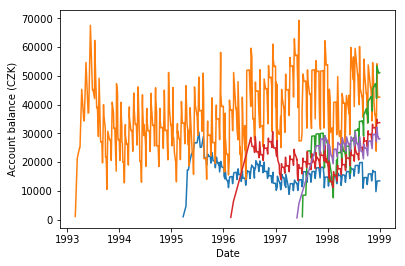
\includegraphics[width=0.45\textwidth]{uploads/upload_da3aa4323224fb439f8fdd1c35ccf4ce.png} &
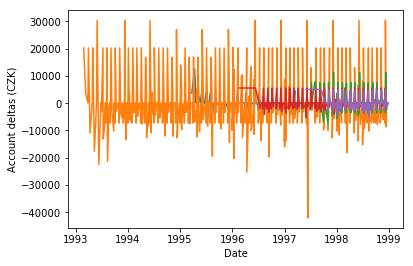
\includegraphics[width=0.45\textwidth]{uploads/upload_8dad9effb8861f12b99f56905a6069fb.png}\tabularnewline
\midrule
\endhead
(a) Account balances & (b) Daily deltas\tabularnewline
\bottomrule
\end{longtable}

Fig. 1: Typical variation in different accounts present in the PKDD
dataset. Figure (a) presents account balances for 5 different accounts
created between 1993 and 1999, and (b) presents the daily variations in
the accounts.

Most of the daily variation is of small magnitude, whereas most of the
income occurs at a fixed period of the month. This time information is
indicative of the main salary associated with each account. Other forms
of capital influx into accounts are also known to be present in the
dataset, the most important of which are monthly loan payouts, pensions
and benefits associated with a given account. Since it's not possible to
disambiguate these quantities nor track changes in these quantities
without further information, only an aggregated mean income was modelled
for each account. The distribution for aggregated mean incomes outputed
by this analysis has profile is shown in
\protect\hyperlink{fig-income-dist}{Figure 2}.

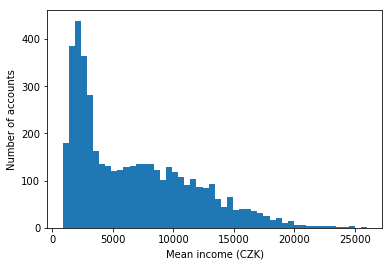
\includegraphics{uploads/upload_948abd778633d8a556ae60e3eaad3a15.png}
Fig. 2: Income distribution estimated for the accounts in the PKDD
dataset.

Applying a similar procedure for expenses associated with each account
yields the profile is shown in
\protect\hyperlink{fig-expend-dist}{Figure 3}.

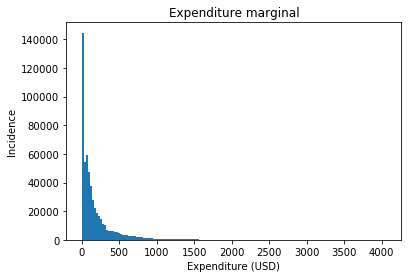
\includegraphics{uploads/upload_cf82f71d41931e913e0484d1f2821767.png}
Fig. 3: Distribution over expenses in the PKDD datasets.



The distributions shown with \protect\hyperlink{fig-income-dist}{Figure
2} and \protect\hyperlink{fig-expend-dist}{Figure 3} can support
probabilistic modeling and guide assumptions to elaborate useful models.

\subsubsection{Merging the PKDD and Government credit card
datasets}\label{merging-the-pkdd-and-government-credit-card-datasets}

Both data sets on their own are insufficient for generating realistic
synthetic data.

The PKDD is comprehensive in the sense that it covers both balance
information and geographical information. However, it does not provide
payement descriptions, which precludes any customer profile modeling.

The Government credit card dataset has complementary information to the
PKDD dataset, that is, it does provide all of the payment descriptions
and amounts charged, but does not have any geographical nor balance
information associated with it.

A possible workaround these issues is to assume that the categories on
which PKDD accounts are spending their capital is similar to those of a
Government area that has simlar spending profile. This concept is
illustrated in \href{fig-matching-profiles}{Figure 4}. To remove
currency effects, the amounts in both datasets were converted to US
dollars.

\begin{longtable}[]{@{}cc@{}}
\toprule
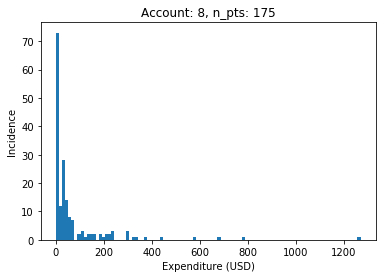
\includegraphics[width=0.45\textwidth]{uploads/upload_45a990d0df922f46b8f78f6bbd3de299.png} &
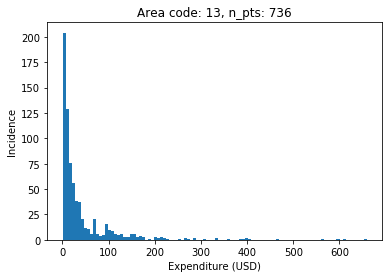
\includegraphics[width=0.45\textwidth]{uploads/upload_65a0e8bbc1a7c9e48a5c07f53fade04c.png}\tabularnewline
\midrule
\endhead
(a) Spending profile associated with PKDD Account 8 & (b) Spending profile for Government area 13\tabularnewline
\bottomrule
\end{longtable}



Fig. 4: Typical example of account that exhibits similar spending
patterns to Government credit cards. (a) Spending profile associated
with PKDD Account 8 and (b) Spending profile for Government area 13.

\paragraph{Matching consumer account behaviour to council
spending}\label{matching-consumer-account-behaviour-to-council-spending}

To fuse both information sources, let \(s\) define the spending
patterns, \(x\) an account and \(y\) a council area.

Then, to match an account in the PKDD dataset to Government credit card
dataset, find \[
(i^{\star}, j^{\star}) = \arg\min_{\substack{i\in \mathcal{I}\\ j\in \mathcal{J}}} \mathrm{KL}
    \big(
        p(s|x=i) \big\| p(s|y=j)
    \big)
\] where \(\mathcal{I}=\{1,\ldots,N\}\), \(\mathcal{J}=\{1,\ldots,M\}\),
\(N\) is the number of accounts in the PKDD dataset and \(M\) is the
number of government areas in the Government credit card data set.

Assuming \(p(s|x=i)\) and \(p(s|y=j)\) are exponential-family
distributions, the Kullback-Leibler divergence minimisation reduces to
finding the government area distribution whose moments most closely
match to those of a given PKDD dataset account.

This procedure can be efficiently implemented by computing a moment
vector \(v\) with mean, variance, skewness and kurtosis of the
distributions associated with both the PKDD dataset and the government
credit cards, then selecting the \((i^{\star}, j^{\star})\) pairs such
that

\[
   (i^{\star}, j^{\star}) = \arg\min_{\substack{i\in \mathcal{I}\\ j\in \mathcal{J}}}
    \big\|
        v_{p(s|x=i)} - v_{p(s|y=j)}
    \big\|.
\]

\paragraph{Imputing expenditure
categories}\label{imputing-expenditure-categories}

To perform missing data imputation based on the pairs
\((i^{\star}, j^{\star})\), a model for the missingness needs to be
chosen. The canonical choice for this case is to employ a clustering
algorithm, such as the mixture of Gaussians.

In the mixture of Gaussians model, the probability that a missing label
\(c\) is equal to label \(k\) is given through Bayes rule as
\[p(c=k|s) = \frac{p(s|c=k)p(c=k)}{p(s)}\] where \(p(c)\) is categorical
and \(p(s|c)\) is a mixture of Gaussians such that

\[ p(c = k)= \pi_{k} \]

\[ p(s|c_{i}) = \mathcal{N}(s; \mu_{i}, \sigma_{i}^{2}) \]

\[ p(s) = \sum_{i=1} \pi_{i} \mathcal{N}(s; \mu_{i}, \sigma_{i}^{2}) \]

Because in the specific case analysed all clusters are already observed
and need not be learned, we can directly estimate each of the parameters
directly without needing to resort to more complex models. This
procedure yielded the category spending distribution for PKDD acconts
shown in \href{fig-matching-cats}{Figure 5}.

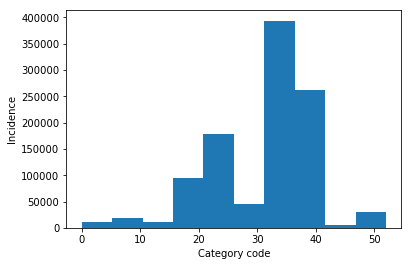
\includegraphics{uploads/upload_de507def2e1d259af1edaaf5812ca5ae.png}
Fig. 5: Category distribution over inputed data.

Additional metadata for each transaction was also inputed in a second
step. The payees for a given transaction were modelled as a multinomial
distribution conditioned on a given category and sampled for different
transactions. This procedure was adopted due to the project's time
constraints and to highlight a possible different approach. However, the
same procedure used for category allocation can also be employed.

\section{Probabilistic data
generator}\label{probabilistic-data-generator}

Probabilistic generative models specify the data generating mechanism as
a composition of random variables. Probabilistic generative models are a
very useful tool as they can translate our assumptions and prior
knowledge about the data into a probabilistically sound framework. This
permits generic approaches such as MLE, or (approximate) Bayesian
inference to learn the model. The assumed structure leads to greater
statistical efficiency and ensures required constraints are obeyed.
Moreover, once the model is learned, probabilistic models allow us to
generate data that is statistically similar to the observed data.

\subsection*{Overview}

The algorithm proceeds in a pre-determined structure where stochastic
choices are made at each stage: 
\begin{itemize}
    \tightlist
    \item \texttt{For\ each\ customer:}
    \begin{itemize}
    \tightlist
    \item Generate customer from a prior distribution over customer attributes.
These are readily available from the ONS although covariances may need
to be modelled in-house. Examples:
    \begin{itemize}
        \tightlist
        \item Geographic location (incl. crime rate, house prices, average age, \ldots{})
        \item Salary
        \item Age
        \item \ldots
    \end{itemize}
    \item Conditioned on the above, sample a distribution over transaction types.
    \end{itemize}
    \item \texttt{For\ each\ transaction:}
    \begin{itemize}
        \tightlist
        \item Sample a transaction cluster
        \item Sample a transaction type from the selected cluster
        \item Sample a transaction amount conditioned on the transaction type and customer
attributes.
    \end{itemize}
\end{itemize}

The path of the data generation process is carefully chosen to ensure the
minimal difficulty learning conditional distributions. In this section
we will first discuss our initial thoughts, a couple of (now) classical
probabilistic models that are used in the development, and then consider
the full probabilistic model. Creating a sensible time series from these
transactions will be left to section 4.

\subsection{A Simple Transaction Model}\label{a-simple-transaction-model}

This model represents our first pass at a generative model for
transaction generation. We specified a probabilistic graphical model
that encoded some minimal structural features of the dataset -- see
Figure \ref{fig:simple_model_sketch}. It primarily ensures that customers have different
distributions over transactions given their age, salary and location. It
is specified as follows:

\begin{itemize}
\tightlist
\item
  Draw \(W \sim N(\boldsymbol 0,\text{diag}(\lambda))\)
\item
  For \(k\in\{1,\dots,\}\), sample
  \(\phi_k^\alpha \sim \text{Exp}(\eta)\) and
  \(\phi_k^\beta \sim \text{Exp}(\zeta)\)
\item
  For each customer \(i \in \{1,\dots,I\}\) with features \(b_i\)
  derived information such as salary and location.

  \begin{itemize}
  \tightlist
  \item
    Calculate \(\theta_i = \text{softmax}(W b_i)\). This vector
    represents the proportion of transaction types for each customer.
  \item
    For each transaction \(j \in \{1,\dots,J\}\), sample a transaction
    type \(y_{ij}\sim\text{categorical}(\theta_i)\).
  \item
    For each transaction \(j \in \{1,\dots,J\}\), sample a transaction
    amount
    \(x_{ij}\sim\text{Gamma}(\theta_i^T\phi^\alpha, \theta_i^T\phi^\beta)\).
  \end{itemize}
\end{itemize}

\begin{figure}
    \centering
    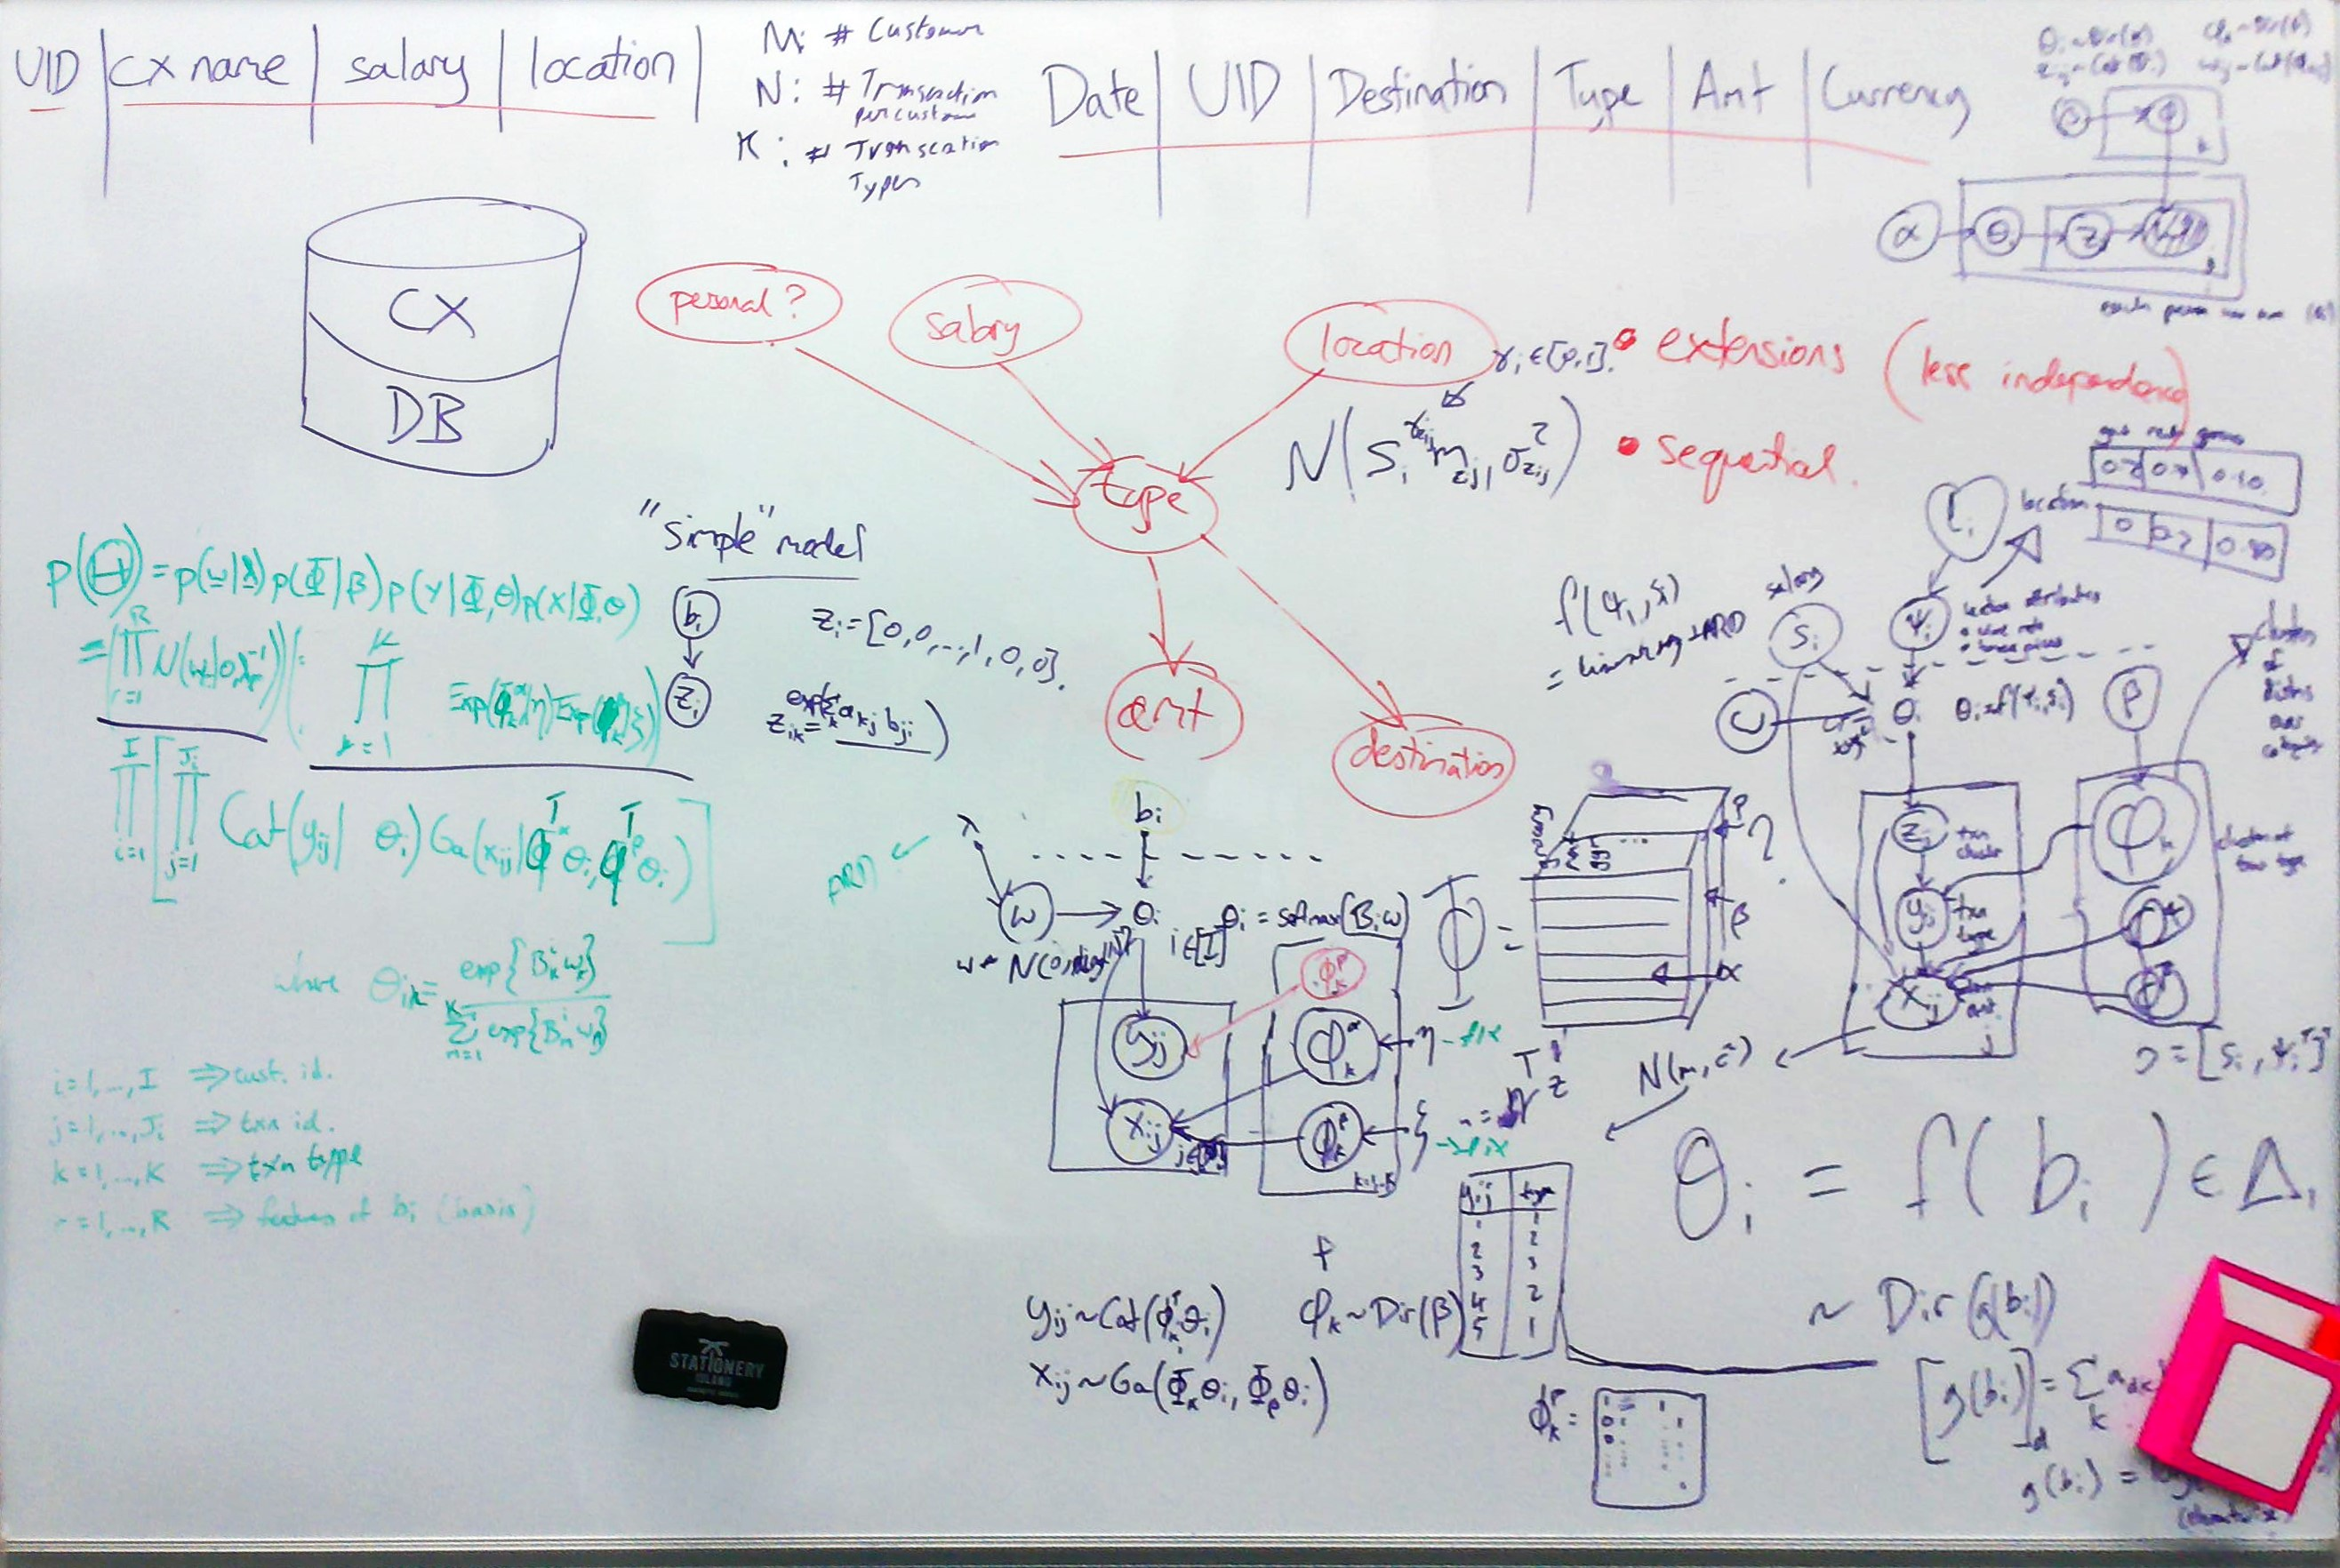
\includegraphics{uploads/upload_f3cde5816b6bbcecbbdc3436ed9f3b34.jpg}
    \caption{The original model sketches made in the group. We seek to
encode the relationships implied by the red graph.}
    \label{fig:simple_model_sketch}
\end{figure}

\begin{figure}
    \centering
    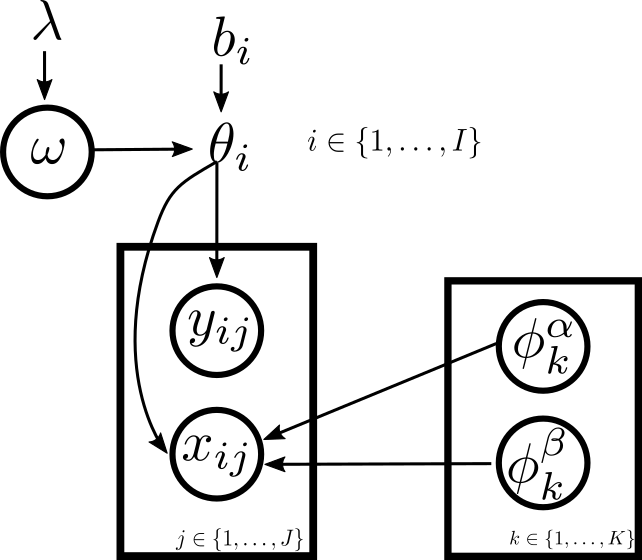
\includegraphics{uploads/upload_33fde9a71f5f4e52d8c44158e39937df.png}
    \caption{The corresponding graphical model to Figure \ref{fig:simple_model_sketch}}
    \label{fig:simple_model_sketch}
\end{figure}


The following is an implementation of the model is Stan (a probabilistic
programming language):

\begin{verbatim}
data{
    int I;
    int R;
    int K;
    real eta;
    real zeta;
    int J;
    real x[I, J];
    vector[R] b[I];
    matrix[K,R] lambda;
}
parameters{
    matrix[K,R] omega;
    vector<lower=0>[K] phi_alpha;
    vector<lower=0>[K] phi_beta;
}
transformed parameters{
    simplex[K] theta[I];
    for (i in 1:I){
        theta[i] = softmax(omega*b[i]);
    }
}
model{
    for (k in 1:K){
        for (r in 1:R){
            omega[k,r] ~ normal(0, lambda[k,r]);    //prior
        }
    }
    for (k in 1:K){
        phi_alpha[k] ~ exponential(eta);    //prior
    }
    for (k in 1:K){
        phi_beta[k] ~ exponential(zeta);    //prior
    }
    for (i in 1:I){
        for (j in 1:J){
            x[i,j] ~ gamma(dot_product(phi_alpha, theta[i]),dot_product(phi_beta, theta[i]));
        }
    }
    for (i in 1:I){
        for (j in 1:J){
            real prob_state[K];
            for (k in 1:K){
                prob_state[k] = log(theta[i, k]);
            }
            increment_log_prob(log_sum_exp(prob_state));
        }
    }
}
\end{verbatim}

The implementation of this model in Stan is subtle, since the discrete
variables must be (analytically) integrated out. The internal inference
engine (variants of Hamiltonian Monte Carlo) is only applicable to
discrete variables.

Since the model implies a fixed mean and variance per transaction type,
and an extremely large space of transaction types, we do not believe
useful parameters and samples can be generated from this model.

\subsection{Use of Existing Models}\label{use-of-existing-models}

\subsubsection{Latent Dirichlet
Allocation}\label{latent-dirichlet-allocation}

Latent Dirichlet Allocation (LDA){[}\^{}blei{]} is a probabilistic
generative model often used to infer topics in word documents in an
unsupervised framework. More generally, LDA learns to categorise sets of
observations into latent clusters of which each document represents a
mixture. It may alternatively be thought of as related to Probabilistic
Latent Semantic Analysis (PLSA) or discrete matrix factorisation.

For the purpose of generating transactions data, LDA can be used to
infer the type of transactions in an exisiting dataset. It can also be
used as a model to generate transactions of certain types.

\begin{figure}
    \centering
    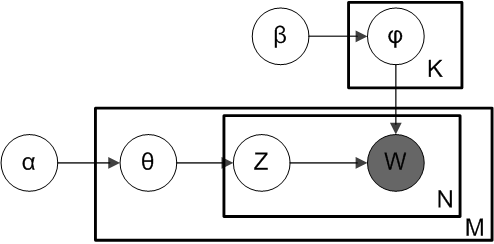
\includegraphics[width=0.6\textwidth]{uploads/Smoothed_LDA.png}
    \caption{Latent Dirichlet Allocation (see \citep{blei2003latent}). Image credit belongs to Wikimedia Commons (https://upload.wikimedia.org/wikipedia/commons/4/4d/Smoothed\_LDA.png)}
    \label{fig:lda}
\end{figure}

\subsubsection{Gaussian Process
Regression}\label{gaussian-process-regression}

Gaussian Processes (GPs) are flexible non-parametric models that can be
used as regression models. A GP is a collection of random variables, any
finite number of which is jointly Gaussian {[}Rasmussen and Williams
2006{]}. To fit a Gaussian Process Regression Model, one only needs to
specify a covariance structure that describes the covariance between the
random variables (outputs). Being Bayesian models, GPs have the
advantage of allowing to incorporate prior knowledge into the model, as
well as quantifying the uncertainty in its predictions.

\begin{figure}
\centering
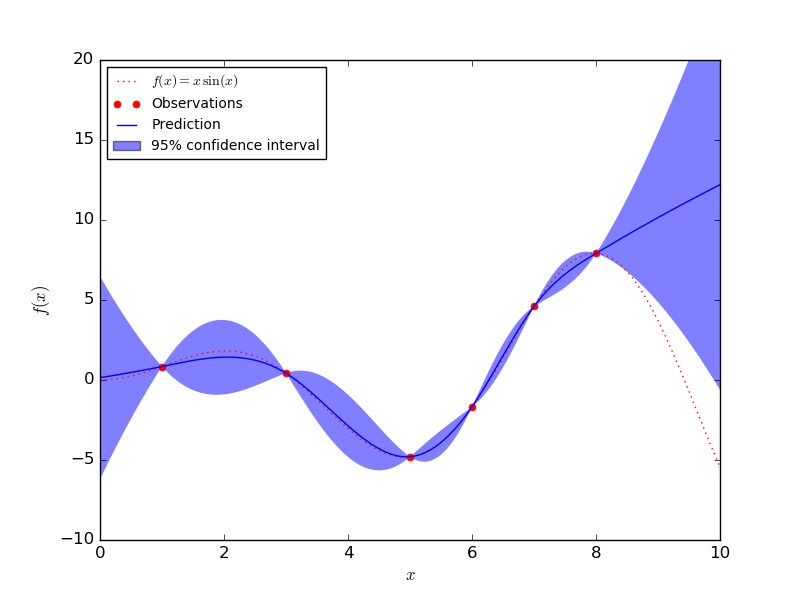
\includegraphics[width=0.6\textwidth]{uploads/plot_gp_regression_001.png}
\caption{Gaussian Process Regression. Image credit: Sci-kit Learn.}
\label{fig:gp_canonical}
\end{figure}

\paragraph{GPs for Transaction Amount
modelling}\label{gps-for-transaction-amount-modelling}

Since GPs are flexible function approximators as well as probabilistic
models, it is possible to fit fairly arbitrary relationships between
variables, as well as sample from the posterior distribution. In this
section we consider relaxing the strong assumption made on transaction
amount (constant mean and variance per transaction type) in the first
transaction model.

\paragraph{Using the Augmented
Data}\label{using-the-augmented-data}

In order to test the validity of the model, we test using the customer
information and transaction types from the augmented dataset described
in section 2.1. As inputs we used four customer attributes: mean income,
inhabitants, and crime rate of the local area, and inferred income of
the customer. These were motivated purely by availability of the data.
The inputs were used to predict the monetary amount of each transaction.

\paragraph{Training}\label{training}

We build a seperate GP model for each transaction type. For performance
reasons, each category was downsampled to 2000 customers and used to
train a GP. An example of the predictive performance of the GP is given
in the figure below:

\begin{figure}
\centering
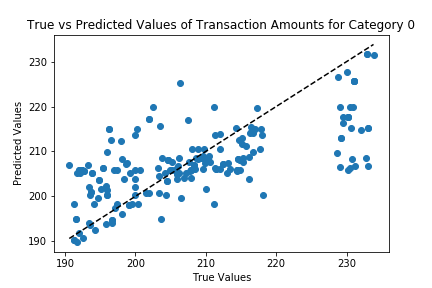
\includegraphics{uploads/upload_293f576878604f4f3bcc81bbe9e07422.png}
\caption{Training error of GP transaction amount prediction for Category 0. $R^2 = 0.45$.}
\label{fig:gp_predict_error}
\end{figure}


% \begin{verbatim}
% // TO IGNORE // ##### 2.3.1.4 Data Generation
% To generate transactions data from the GP model, we sample demographic information and salary from the dataset. Next, we randomly choose a transaction type from a prespecified distribution. We pick the GP that corresponds to the transaction type that was selected and feed it the demographic and salary information to obtain a posterior distribution. Finally, we sample from the posterior distribution to obtain a transaction amount.
% \end{verbatim}

\paragraph{Limitations}\label{limitations}

A particular scale length of the kernel must be chosen (e.g.~by marginal
likelihood). However, it is not always the case that a single scale
length is appropriate for the entire support. It has also been noted
that some types of data (particularly images) exhibit highly nonlinear
manifolds, which will be oversmoothed by GPs.

\subsection{Proposed Probabilistic
Model}\label{proposed-probabilistic-model}

The following full model is given for modelling the transactions and
amounts of various types of customers. In order to reduce clutter, the
plate over \(i\) (that is, the customer ID), has been omitted. Where
relevant, the random variables should be assumed duplicated. The
variables interpretations are annotated in red.

\begin{figure}
    \centering
    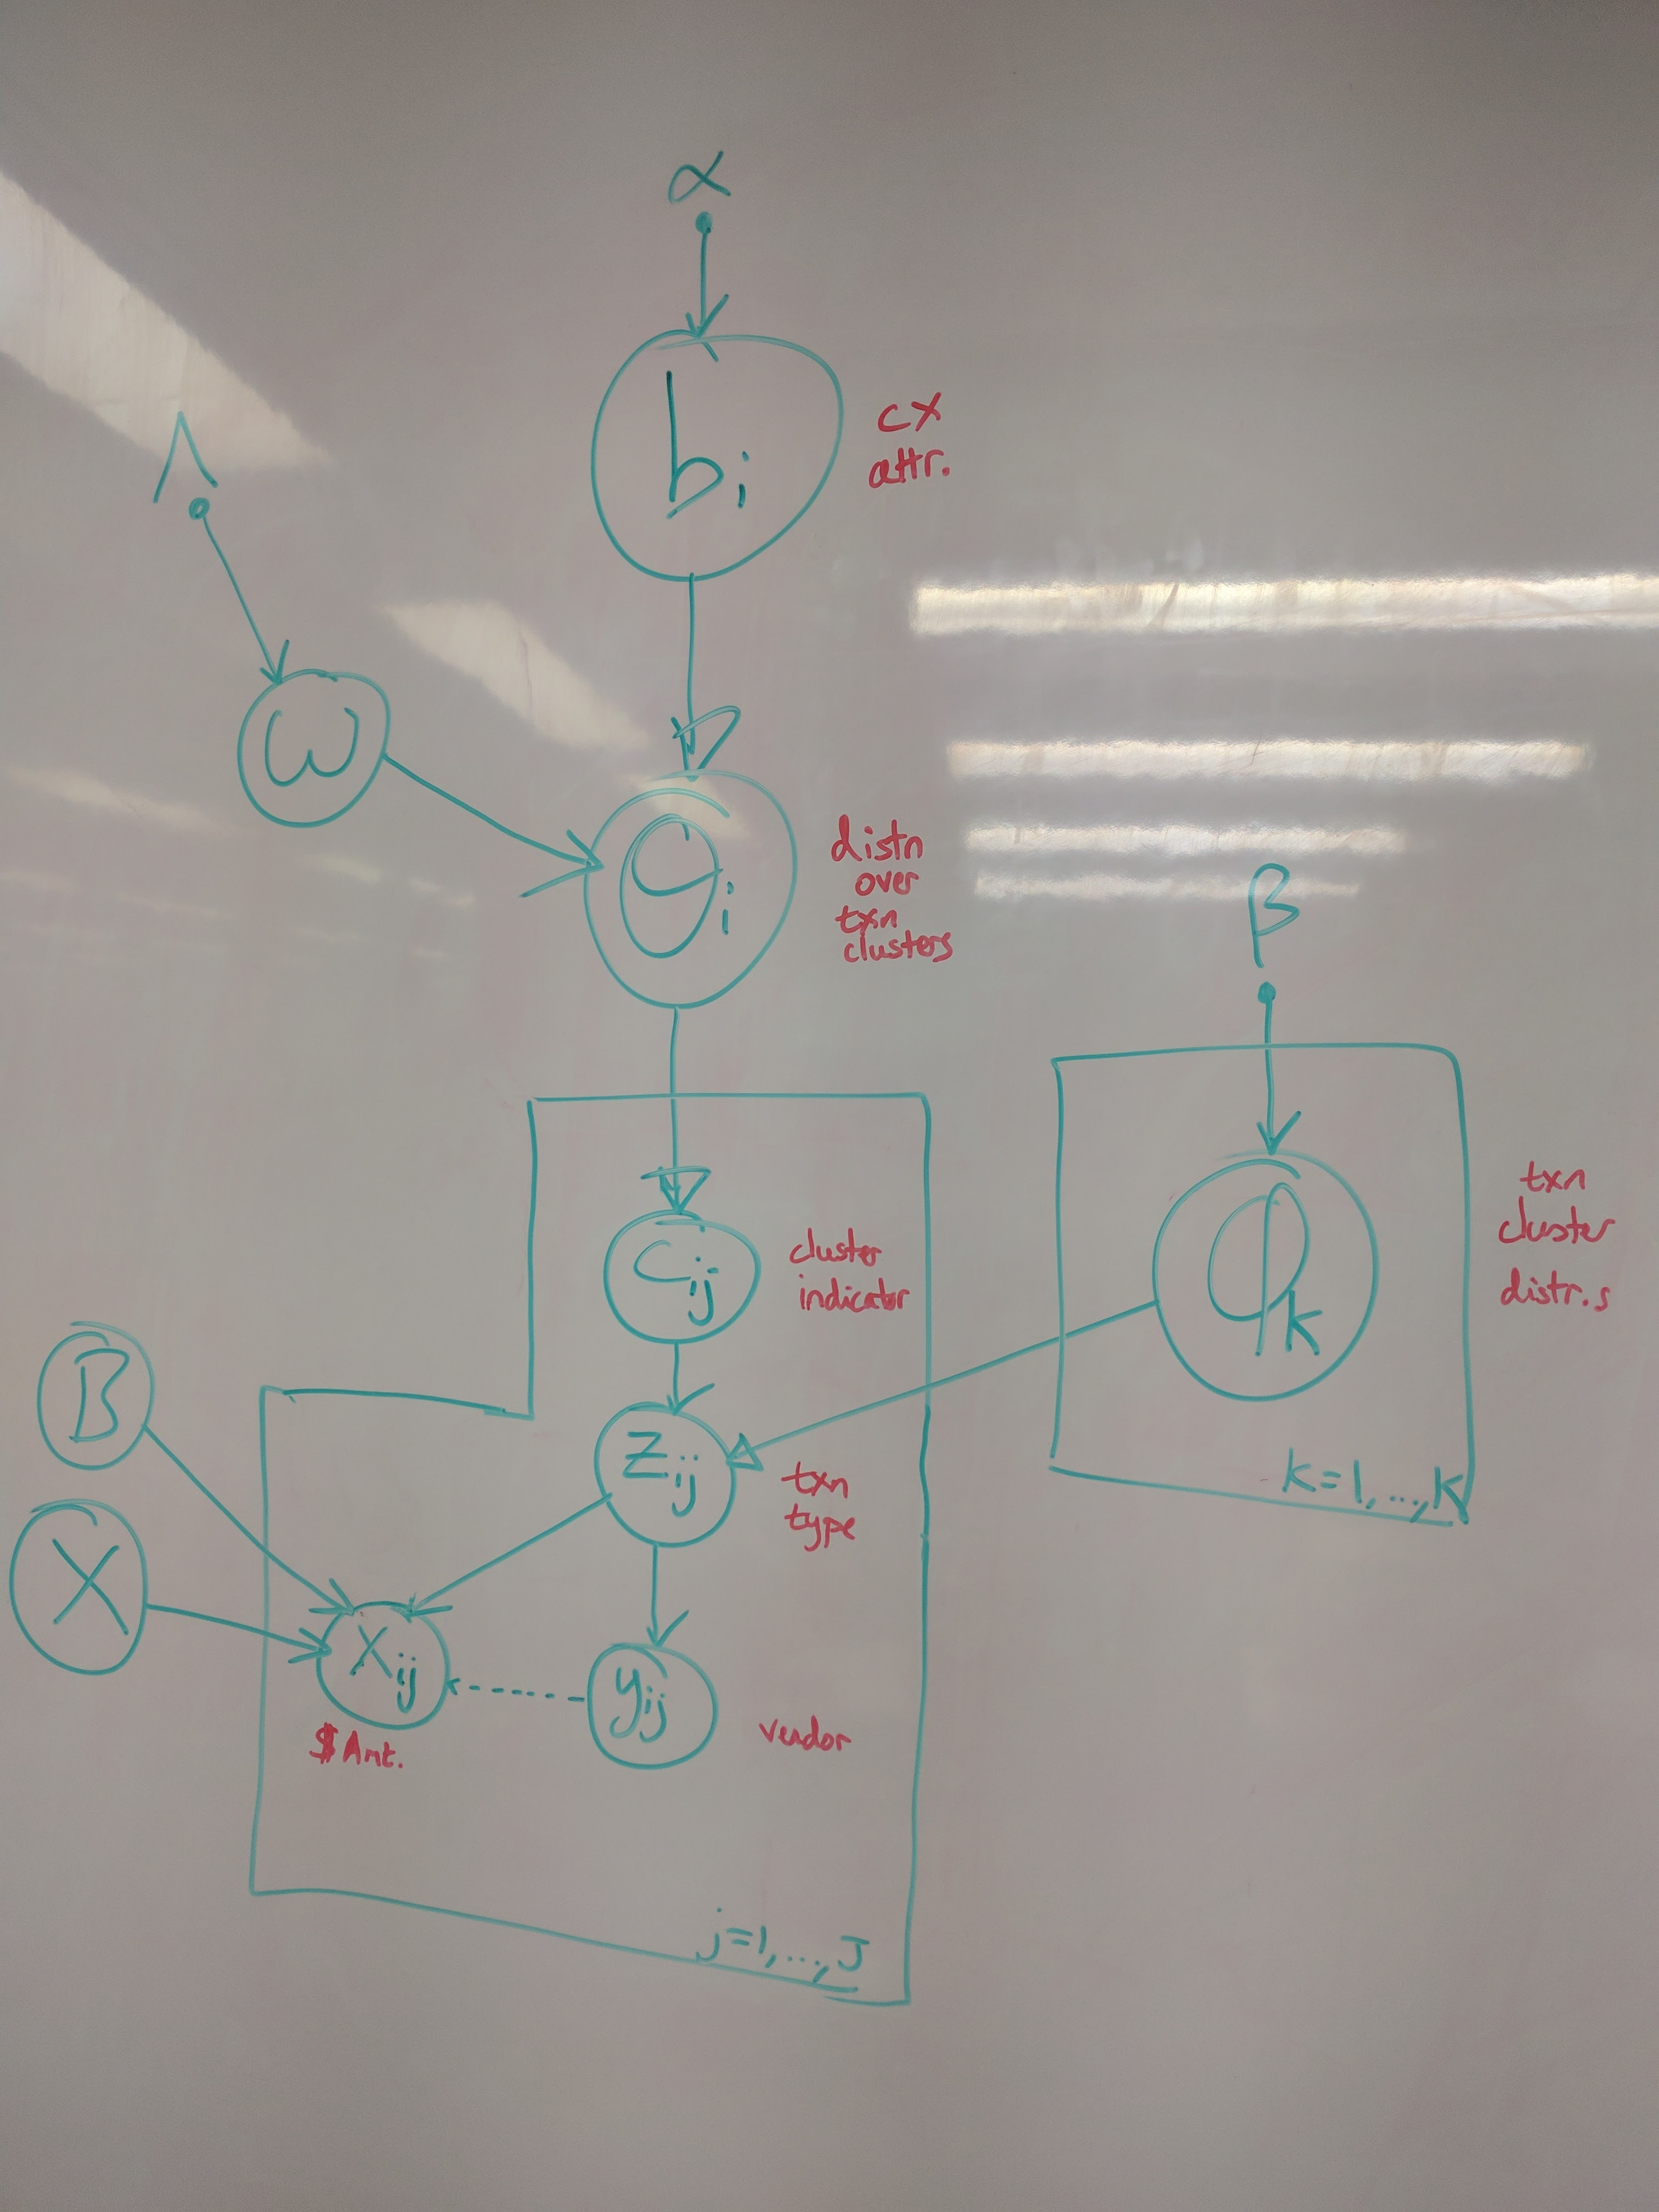
\includegraphics[height=0.8\textheight]{uploads/upload_37fb8c8385fe1a4fc0231ccb4dee1d28.jpg}
    \caption{Proposed Probabilistic Model}
    \label{fig:proposed_model_sketch}
\end{figure}

We observe the amounts \(x_{ij}\) and vendors \(y_{ij}\), and possibly
the transaction types \(z_{ij}\). We further assume that the customer
features \(b_i\) are observed. The distributions suggested are:
\begin{align*}    
b_i &\sim p(\alpha) \\
\theta_i &\sim \text{Dir}(W b_i) \\
\phi_k &\sim \text{Dir}(\beta) \\
c_{ij} &\sim \text{Cat}(\theta_i) \\
z_{ij} &\sim \text{Cat}(\phi_{c_{ij}}) \\
y_{ij} &\sim \text{Cat}(\gamma_{z_ij}) \\
x_{ij} &\sim \mathcal{GP}(B, X)
\end{align*}
One may observe that it is similar in principle to the supervised LDA
model given in the previous section. However, a number of additions have
been made. 
\begin{enumerate}
    \tightlist
    \item The cluster parameters \(\phi_k\) now correspond to
\emph{distributions} over transaction types. Thus when modelling large
numbers of transaction types, clusters will be automatically determined
by the model. This should correspond to a meaningful quantity such as
supermarkets, or takeaways, utility companies etc. This means that
individual companies need not be modelled separately, but are grouped
automatically with similar organisations. 
    \item An additional vendor
realisation \(y_{ij}\) is given, in case one wishes to model different
types of the same vendor (different location, branch, umbrella, etc.).
    \item \(x_{ij}\) is modelled in a more flexible way: one recommendation is
to use GPs. Of course this makes the model much more difficult to learn
-- see next section.
\end{enumerate}

The vector \(b_i\) of customer attributes can only consist of the same 4
attributes given as inputs in the GP model, and derived features thereof
(powers, reciprocals, products, \ldots{}). However the power of the
model will be enhanced where more customer data is available to explain
variations in behaviour. On the other hand, if greater privacy is
desired, it may be advantageous to remove some elements of this vector.

\subsubsection{Approximation to Proposed
Model}\label{approximation-to-proposed-model}

Performing inference and learning in the previous model is extremely
challenging, and is out of scope for a 3-4 day study group. However, we
can form an approximation to the model by learning the topic model by
learning the LDA submodel without the supervision, and assuming the
transaction amount is unobserved (or contains no information about the
transaction type). See below picture:

\begin{figure}
    \centering
    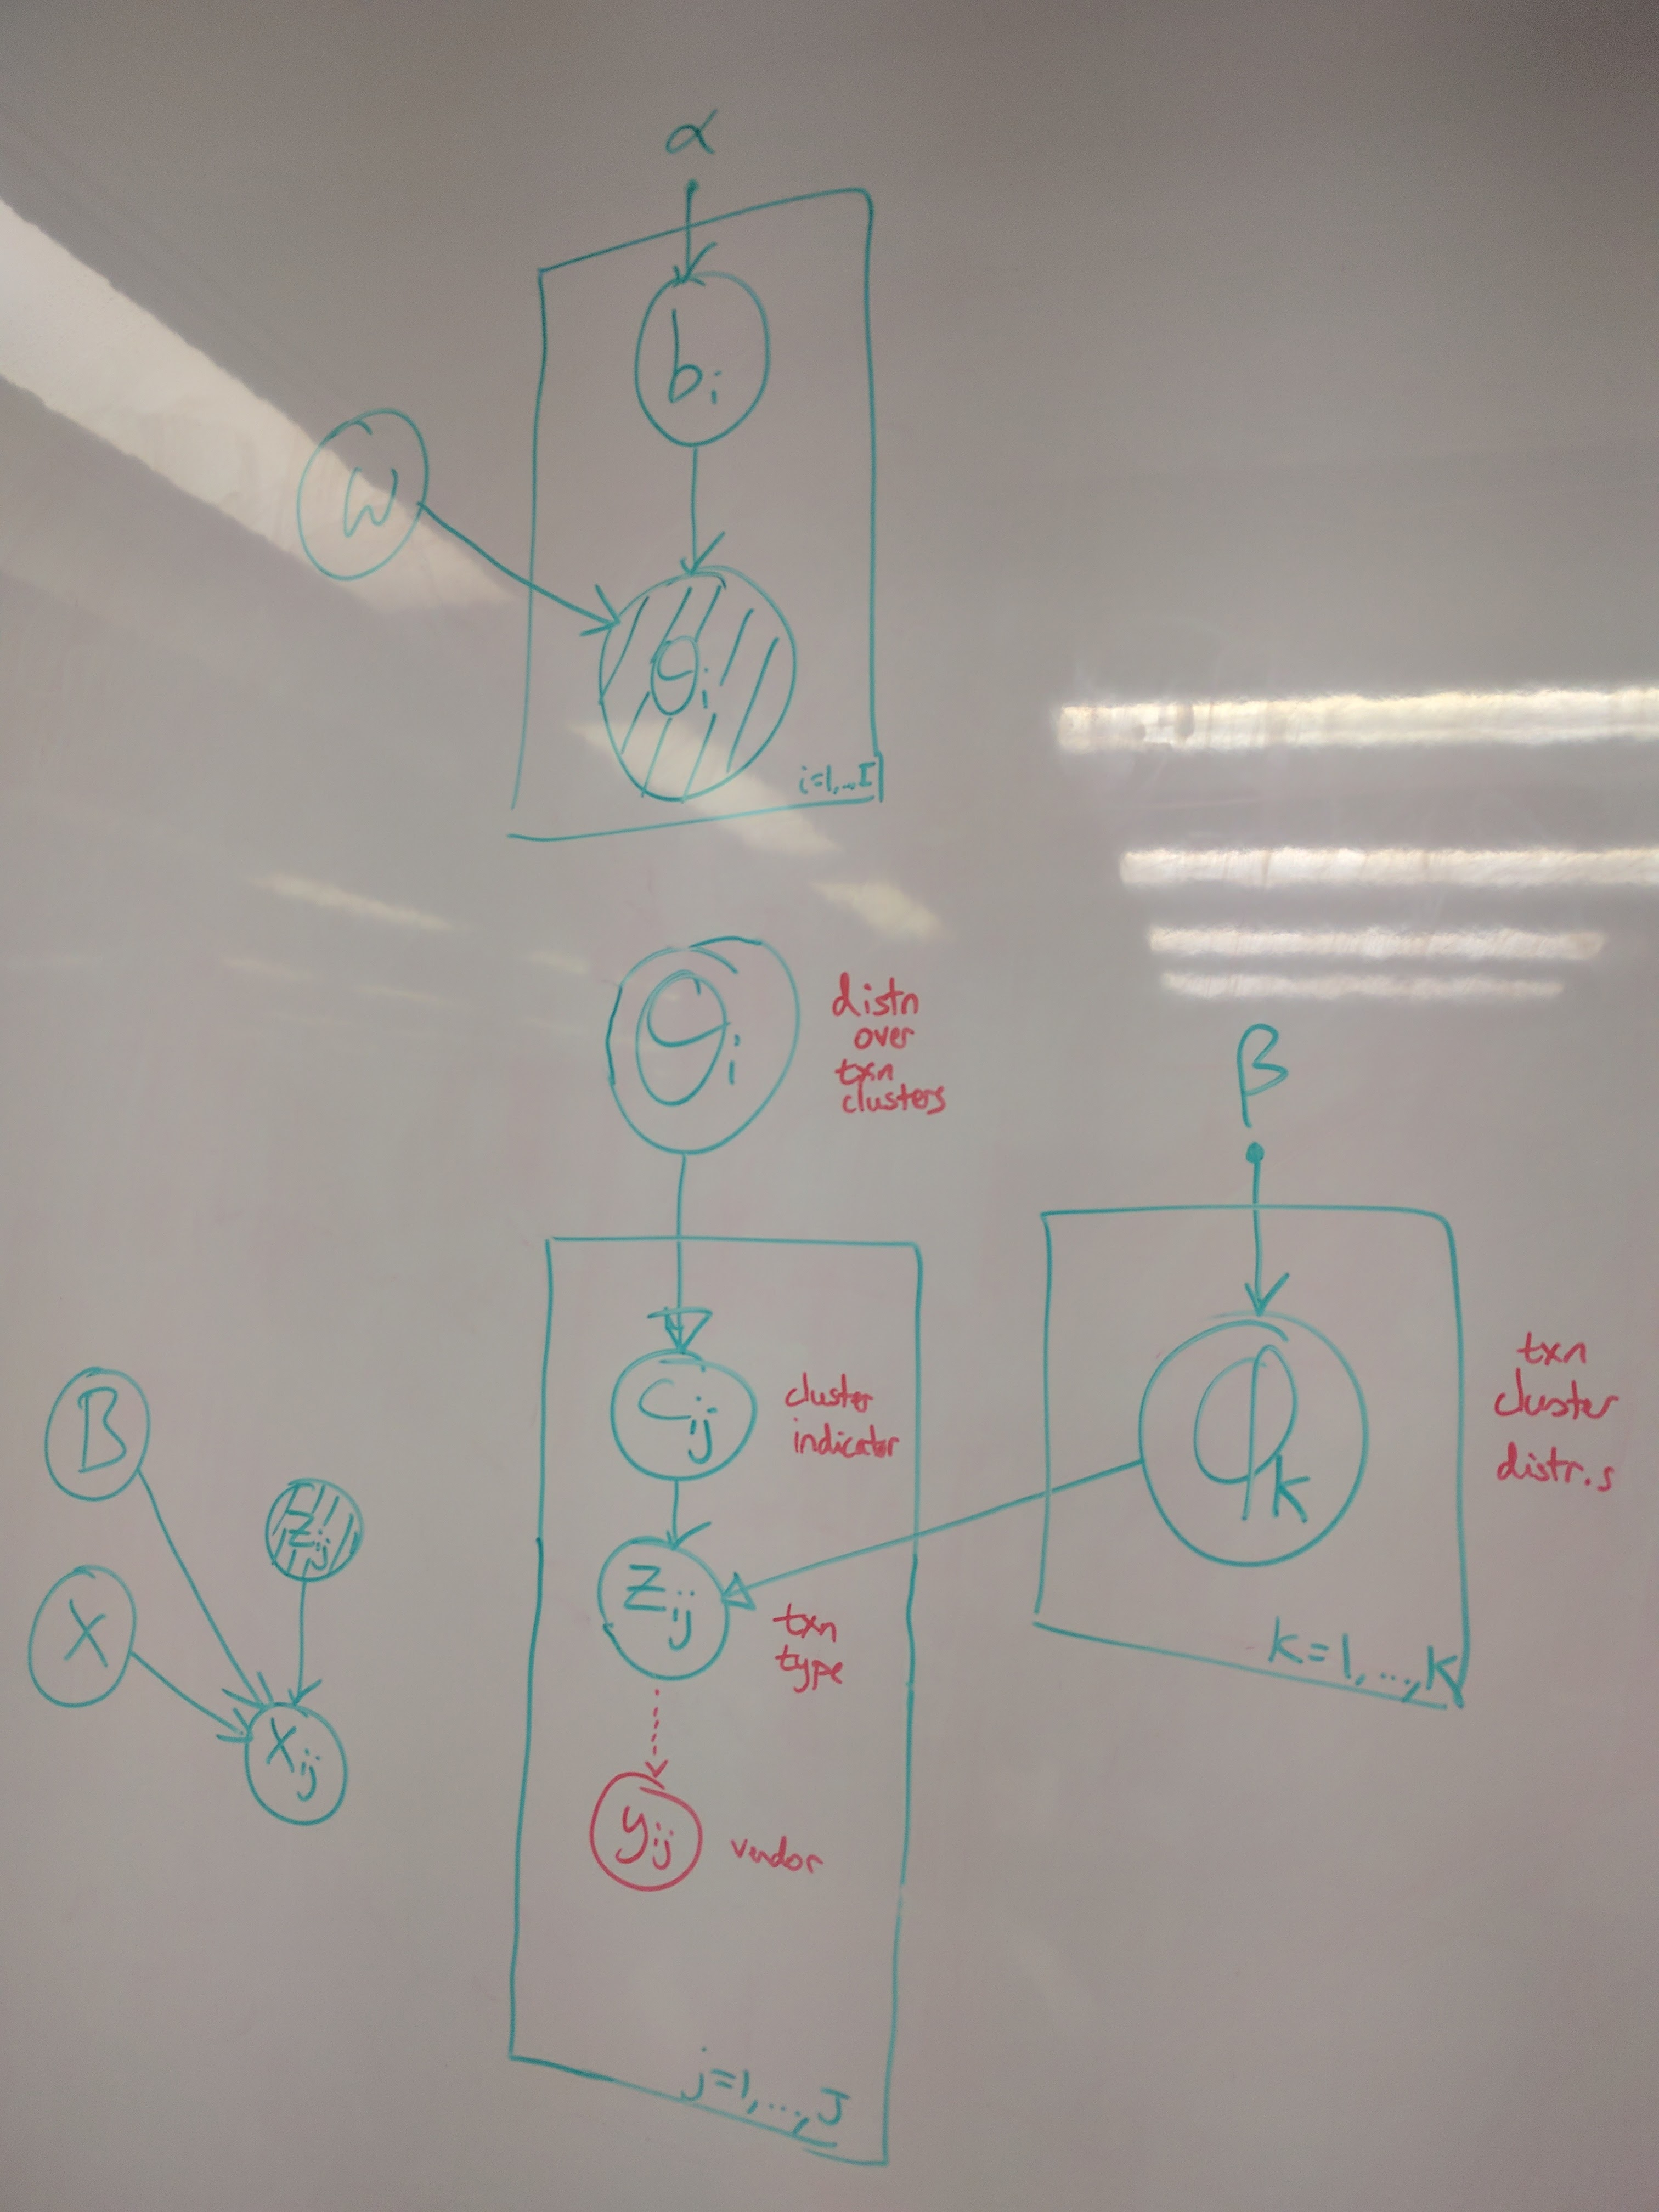
\includegraphics[height=0.8\textheight]{uploads/upload_0f89a47727b7b7c85cf6125f76474d5c.jpg}
    \caption{Approximation to Proposed Probabilistic Model, c.f. Figure \ref{fig:proposed_model_sketch} }
    \label{fig:proposed_model_approx}
\end{figure}

Suboptimality will arise in 2 obvious ways from this choice. Firstly in
a similar way to approximations of mixture-of-experts models, the
clusters learned will not be optimal for the information gained from the
supervision. (The clusters are useful for description, not prediction
given the customer attributes.) Secondly by including information from
transaction amount, high-end vs inexpensive distinctions may be better
made in cluster type.

Nevertheless, the efficiency gains made in inference and learning are
substantial. The model can be learned in the following steps:

\begin{enumerate}
\def\labelenumi{\arabic{enumi}.}
\tightlist
\item
  Perform LDA across transaction and customers to learn the \(\phi_k\)
  and \(\theta_i\).
\item
  Perform ``softmax'' regression on the \(\theta_i\).
\item
  Create a GP model for the \(x_{ij}\) as explained in section 3.2.
\end{enumerate}

Data can then be generated by first simulating from some joint
distribution over customer features (for instance, a simple model might
be to use marginal distributions from ONS, and assume independence), and
then sampling from the model given above.

\subsubsection{Predicting categorical
distributions}\label{predicting-categorical-distributions}

We may observe that step (2) is essentially an MLP (Neural Network) with
no hidden layers. Thus, while a neural network does not learn parameters
that ensure the output distribution is faithful to these probabilistic
semantics, the gain in function approximation may be well worth the
experiment.

Small experiments have been performed in this group which have resulted
in extreme low entropy outputs (one-hot vectors). An intuition behind
this outcome is that the neural network is extremely sensitive to
initialisation for predicting distributions. The softmax layer can be
seen as a competition between competing categories, where the winner
(the largest value) takes all. Only when all values are relatively small
can the softmax emit a high entropy distribution. The relative parameter
values may result in gradient descent following an increasing path in
pre-softmax output values.

While it is not an entirely unexplored space for research, the authors
of this report have not uncovered significant work on generic supervised
methods for predicting categorical distributions. This area may require
more time and research to explore thoroughly.

\paragraph{Output and Discussion}\label{output-and-discussion}

The major output of this model will be a customised categorical
distribution over transaction cluster types and/or vendors. Provided
sufficient training data is given, we have high confidence that these
distributions can capture fairly sophisticated relationships between
customer (including business) types and the names and amounts of
transactions made on their account. Very few significant assumptions are
made in the model which would deteriorate performance; provided the
topic-model-type decomposition is valid over transactions, categorical
distributions are able to capture arbitrary distributions, and GPs are
also extremely flexible.

Unfortunately we are unable to provide a complete end-to-end
implementation of the above approximation. The MLP implementation
currently fails to give distributions as output. Nevertheless, due to
the nature of the training data, there was almost no signal in the data
to learn, so following the GIGO principle, it would not have anyway been
a fruitful endeavour. Code for all stages may be found in the code base
attached.

\section{Agent Based Models}\label{agent-based-models}

An agent-based model (ABM) {[}1{]}, {[}2{]}, {[}3{]}, {[}4{]} is a
computational model for simulating the actions and interactions of
autonomous agents (in our case, customers and suppliers) with a view to
assessing their effects on the financial transaction system as a
whole{[}5{]}. ABM is a powerful simulation modelling technique in which
each agent assesses the situation and makes decisions on the basis of a
set of rules. Agents may execute various behaviours that are appropriate
for the environment they represent{[}6{]} . Even a simple agent-based
model can exhibit complex behaviour patterns and provide valuable
information about the dynamics of the real-world system that it
emulates{[}6{]}.

ABM captures emergent phenomena, the associated behaviours and provides
a natural description of a system. In many cases, ABM is most natural
for describing and simulating a system composed of ``behavioural''
entities{[}6{]}. In our case, we leverage the benefit of ABM in
simulating a transaction system composed of behavioural entities. The
aim is to simulate the customer transaction behaviours and generate
realistic synthetic transaction data based on those behaviours.


\begin{figure}
    \centering
    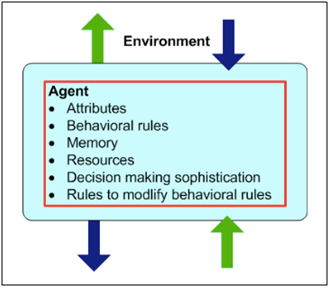
\includegraphics{uploads/upload_294517dbfba011eb51dca1094d201cea.png}
    \caption{An Agent \citep{macal2010tutorial}}
    \label{fig:agent}
\end{figure}

\subsection{When and Why ABM:}\label{when-and-why-abm}

As discussed in the Proceedings of the 2006 Winter Simulation Conference
on `How to model with agents', its important to consider when is it
beneficial to think in terms of agents? {[}7{]} • When there is a
natural representation as agents • When there are decisions and
behaviors that can be defined discretely (with boundaries) • When it is
important that agents adapt and change their behaviors • When it is
important that agents learn and engage in dynamic strategic behaviors •
When it is important that agents have a dynamic relationships with other
agents, and agent relationships form and dissolve • When it is important
that agents form organizations, and adaptation and learning are
important at the organization level • When it is important that agents
have a spatial component to their behaviors and interactions • When the
past is no predictor of the future 

\subsubsection{Toolkit Mesa},
{[}9{]} is a Python framework for agent-based modelling. It allows users
to quickly create agent-based models using built-in core components
(such as spatial grids and agent schedulers) or customized
implementations; visualize them using a browser-based interface; and
analyze their results using python data analysis tools {[}8{]} 

\subsubsection{Building an agent model}
In addition to the standard model building
tasks, ABM requires one to: (a) identify the agents and get a theory of
agent behavior, (b) identify the agent relationships and get a theory of
agent interaction, (c.) get the requisite agent-related data, (d)
validate the agent behavior models in addition to the model as a whole,
and (e) run the model and analyze the output from the standpoint of
linking the micro-scale behaviors of the agents to the macro- scale
behaviors of the system {[}7{]}.

The agent-based modeling toolkit in python provides basic agent
functionality based on the object-oriented paradigm. Agent based
simulation is not the same as object-oriented simulation, but the O-O
modeling paradigm is a useful basis for agent modeling, since an agent
can be considered a self-directed object with the capability to
autonomously choose actions based on the agent's situation. The O-O
paradigm is natural for agent modeling, with its use of object classes
as agent templates and object methods to represent agent behaviors. O-O
modeling takes a data-driven rather than a process-driven perspective.
One way to begin the modeling process is to define abstract data types
and objects {[}7{]}. The general steps in building an agent model are as
follows {[}7{]}: 1. Agents: Identify the agent types and other objects
(classes) along with their attributes. 2. Environment: Define the
environment the agents will live in and interact with. 3. Agent Methods:
Specify the methods by which agent attributes are updated in response to
either agent-to-agent interactions or agent interactions with the
environment. 4. Agent Interactions: Add the methods that control which
agents interact, when they interact, and how they interact during the
simulation. 5. Implementation: Implement the agent model in
computational software.

Identifying agents, accurately specifying their behaviors, and
appropriately representing agent interactions are the keys to developing
useful agent models. Agents are generally the decision-makers in a
system.{[}7{]} A banking customer transaction involves the customer and
the supplier to whom transactions are made. 

\subsubsection{An Illustration}
\paragraph{Premises of the model}\\
The following are assumed available as input:
\begin{itemize}
    \item Categorical Distribution of
types of Supplier
    \item Distribution of spend by transaction type
\end{itemize}

The distribution of the different types of supplier has been modelled as
a categorical distribution which in turn assigns the supplier category
to each of the supplier agents. Furthermore, each supplier has an
intrinsic distribution determining the selling patterns of the seller.
This distribution determines the likely spending of a potential consumer
interacting or visiting the store.

Customer agents execute the following behaviours:

• The customer is credited income every month • The customer is rational
in his spend by monitoring he is not spending in excess of his wealth
and saving by the end of year • The customer can choose a supplier to
spend on • The customer spend is seasonal based on time and special
events • The customer spending preferences are followed Supplier agents
execute the following behaviour: • There are multiple suppliers that
address the needs of the customers • The suppliers are credited the
amount spent by the customer

We begin developing an ABS model by identifying the agent types and
other objects (classes) along with their attributes (Step 1). Each agent
class is represented by a set of attributes and methods that operate on
the agent class. {[}7{]} For example, the customer agent is represented
by the following attributes: the agent's name; unique ID; transaction
types; location and amount spent. The values of these variables at any
point in time constitute the agent state.

We then specify the environment in which the agents live and interact
(Step 2). For example, an environment variable could be the geographic
locale, which could also be included as a customer agent attribute
(Transaction location) {[}7{]}.

We specify the methods by which agent attributes are updated during the
simulation in response to customer agent to supplier agent interactions
or the agent interactions with the environment (Step 3) {[}7{]}.

Add the methods that control which agents interact, when they interact,
and how they interact (Step 4). The agent selection procedure could be
invoked at every time period or when inventory levels reach specified
thresholds. The agent interaction procedure would consist of placing an
order with the selected agent at the determined time {[}7{]}.

The complete set of object class definitions and methods, parameter
values, and initial values for all the agent and other object states
constitutes a complete specification of an agent model. {[}7{]} We
implemented this agent model by writing an object-oriented program
using, Mesa python (Step 5).

\subsubsection{Class diagram}\label{class-diagram}

The UML schema below, succinctly describe the structure of current agent
based model wherein Agent\_Supplier and Agent\_Customer are independent
agent modules governing the behaviour of corresponding behaviours of the
suppliers and the customers while being modelled by the
Transaction\_Model module.

\begin{figure}
\centering
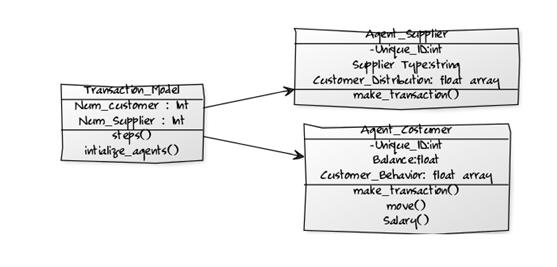
\includegraphics{uploads/upload_33eb3ed0e4788936cb068a5e55703918.png}
\caption{Class diagram for the current implementation}
\end{figure}

\subsubsection{Visualizing the generated
data}\label{visualizing-the-generated-data}

This section analyzes the artificially generated dataset in light of the
standard transactional patterns for the sake of crude statistical
validation of the proposed model. However, the model has been heavily
parameterized by the distribution of the training data and is therefore
likely to portray the statistical fingerprints that of the training
data.

\begin{figure}
\centering
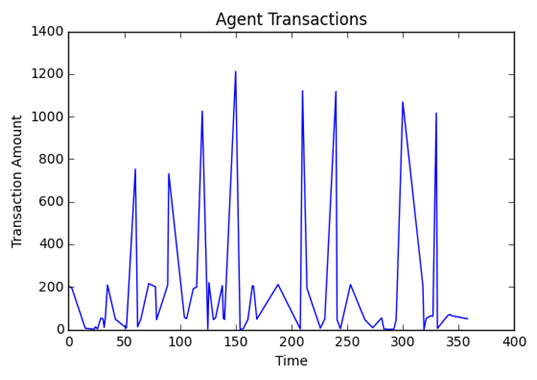
\includegraphics[width=0.6\textwidth]{uploads/upload_8de0984822b859025b78852554b10186.png}
\caption{Agent transactions}
\end{figure}

Figure 3 above portrays the quantum of transaction for a single agent
with regular recurring spikes indicating salary credits. While, Figure 4
portrays the cumulative spendings of all the customers. The figure
further portrays the seasonal nature of the consumer spending habits
with an expected elevation between 300 to 350 time units.

\begin{figure}
\centering
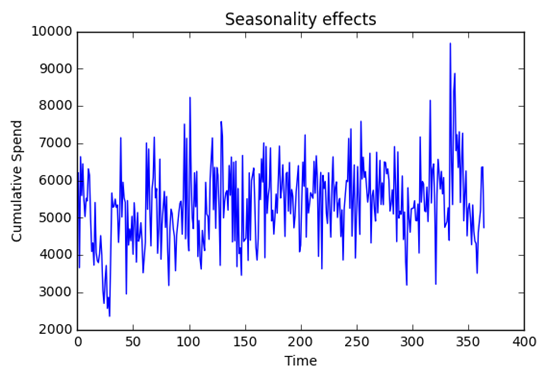
\includegraphics[width=0.6\textwidth]{uploads/upload_5b7adbe2ae9cc4c0a41968d434fcb446.png}
\caption{Cumulative spending behaviour}
\end{figure}

Finally, Figure 5 portrays the credit standings at the end of the term
across the entire customer base. The negative amounts indicate debts
while the a positive amount indicates end of the term savings.

\begin{figure}
\centering
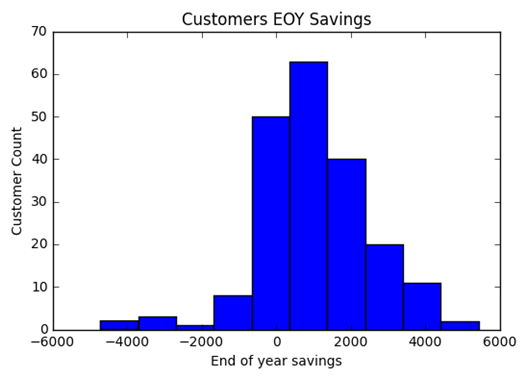
\includegraphics[width=0.6\textwidth]{uploads/upload_f1eb193470c68d9e7f241b3c1bb8c5e9.png}
\caption{End of term credit standings}
\end{figure}

\subsection{Agent based modelling for transaction
prioritization}\label{agent-based-modelling-for-transaction-prioritization}

\paragraph{The purpose}\label{the-purpose}

The purpose of this piece of work is to generate a rational scheme for
how a customer would prioritize his/her expenses as the month goes by.
At each point when a customer would want to make a transaction of some
sort, the probabilistic model for transaction type generation will
provide the uncertainty of the transaction type the customer would
engage, in way of a categorical distribution $\text{Cat}_T$ (Eg. illustrated in
Figure 6).
\begin{figure}
\centering
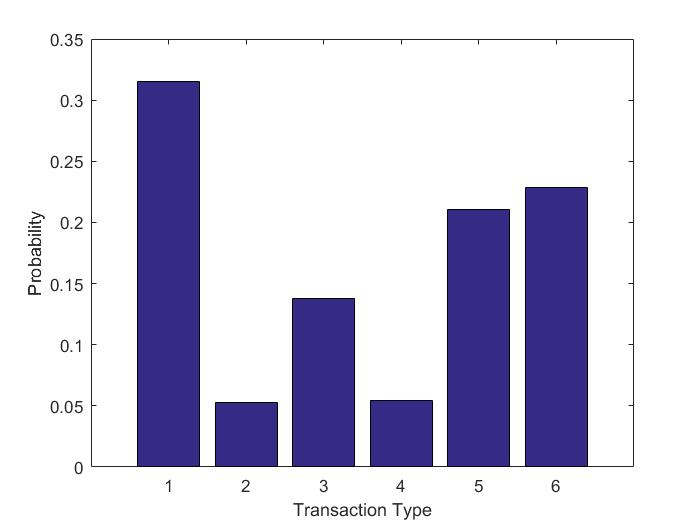
\includegraphics[width=0.6\textwidth]{uploads/upload_f2d5f8e5757a86ec73e739eb5600af0a.jpg}
\caption{Example of a categorical distribution over transaction types}
\end{figure}

The purpose of this algorithm is to define a priority among the
transaction types (Grocery, clothing, holiday, restaurant etc.).

\subsubsection{Markov Decision
Processes}\label{markov-decision-processes}

To accomplish this task, we will try to generate a priority vector that
defines the priority of one transaction type over another. For this we
have to consider the available balance of the customer, what kind of
value would a transaction yield in and most importantly how can the
customer perform a series of transactions without going in to major
debt. To simulate this behaviour we have adopted an agent based
modelling scheme based on Markov Decision Processes (MDP). The states of
the MDP are decided depending on the current bank balance of the
customer as a percentage of his/her total income. The actions on each
time step (i.e.~each time a transaction is made) are defined as
different priority vectors. State transition is defined by the change in
bank balance. An example of the possible state transitions caused by a
priority type (i.e.~an action class within the MDP framework) is
illustrated as in figure 7.

\begin{figure}
\centering
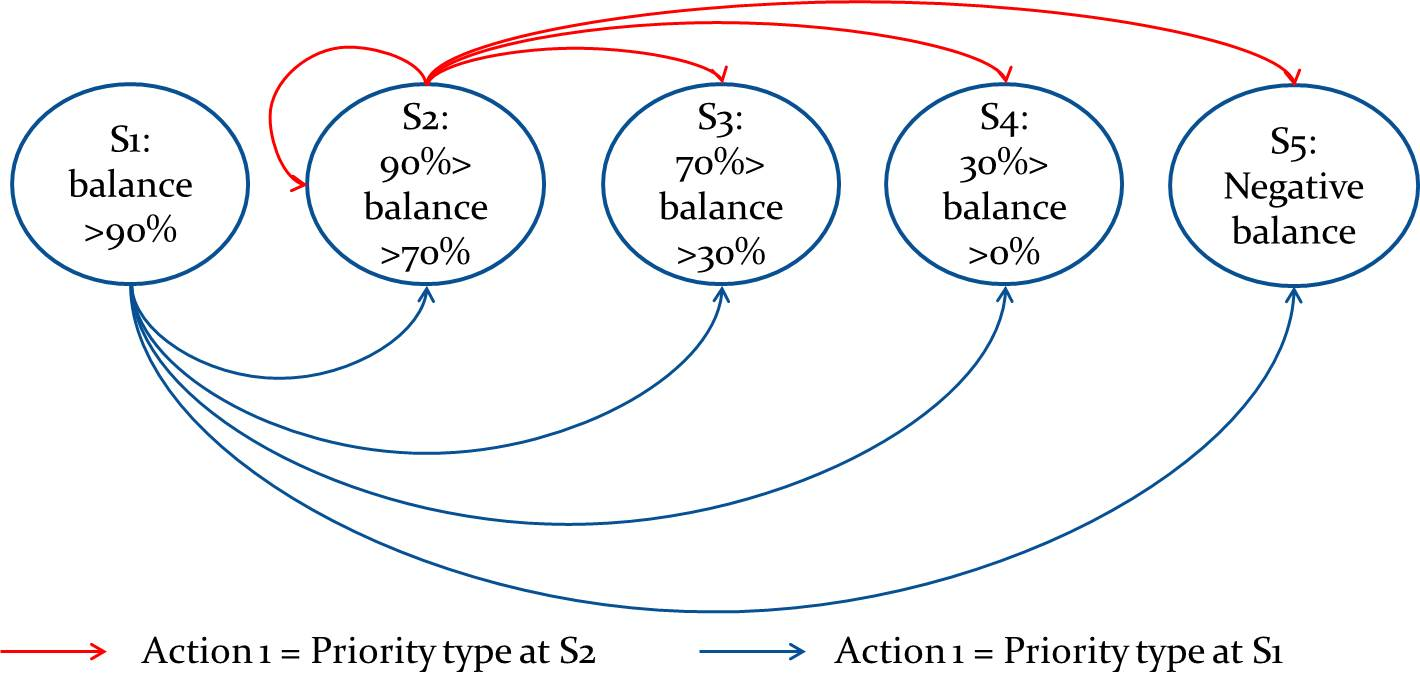
\includegraphics[width=0.5\textwidth]{uploads/upload_d7d1576051453ce269f98a5c597e8bd0.jpg}
\caption{Example of state transitions caused by a action. Note that
each action could result in different transitions due to the stochastic
nature of the transactions}
\end{figure}

\subsubsection{The Algorithm}\label{the-algorithm}

Each action a corresponds to a priority vector $p_T$. According to the $p_T$
selected a transaction Ta, is performed. For this we define a priority
vector $p_T$ over the transaction types, such that higher values correspond
to higher priority, eg. $p_T = [7, 1, 3, 2, 4, 6, 5]/28$, is a priority
vector with the highest priority given to the first transaction type.
The transaction type to perform is sampled from the categorical
distribution $\text{Cat}_T,\text{Adj}$, after adjusting $\text{Cat}_T$ according to the priority
vector $p_T$ as follows:

$$\text{Cat}_T,\text{Adj} = \text{Cat}_T * p_T / \sum (\text{Cat}_T * p_T).$$

Once a transaction type $T$ is identified, the value of the transaction $T_a$
is sampled from corresponding probability distribution of the
transaction type (PDF\textsubscript{T}). For the purposes of this study we assume, that
there exists a PDF\textsubscript{T} that is normally distributed with a mean `mu' and
standard deviation `sigma', for each transaction type $T$, where mu
corresponds to the mean value of the transaction. The mean of this
transaction type can be assumed to vary according to the available
balance. This is to reflect that for a particular transaction, a
customer would be rationally be more conservative when his/her bank
balance is low. For each action a, that the agent performs the agent
receives an immediate reward. The following function assigns rewards to
the agent:

$$R(x,a,y) = \text{transaction\_satisfaction}(T_a) + \text{state\_satisfaction}(y) +
\text{state\_change\_sadness}; $$

Where $R(x,a,y)$ is the immediate reward given to the agent for taking the
action $a$, at state $x$, which transitioned it to state $y$.
transaction\_satisfaction($T_a$) corresponds to the satisfaction the
customer gains by performing the transaction Ta and
state\_satisfaction($y$) corresponds to the satisfaction the customer
gains by being in state $y$ (Eg. customer would be happier to be in states
that correspond to higher bank balances as compared to a negative or low
bank balance). Our target is to generate a sequence of rational actions
(that correspond to priority vectors). To obtain an optimal policy, the
agent cannot only rely only on the immediate rewards, but try to guess
the total future reward. For this purpose we define a future reward
function $Q(s,a)$ , that calculates the maximum expected future reward
that can be obtained for performing action $a$, in state $s$. In our study,
we have implemented this as a table with states as rows and actions as
columns. $Q(s,a)$ function can be iteratively approximated using Bellman's
equations. The algorithm to learn the $Q$ function can be given as follows
{[}11{]}:

\begin{figure}
\centering
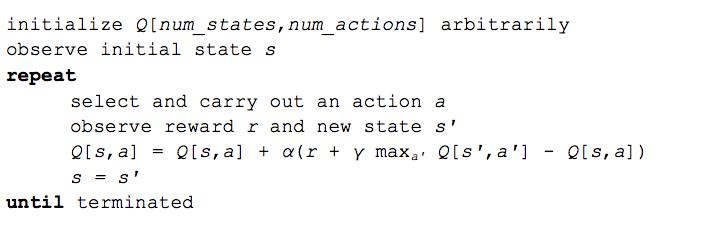
\includegraphics[width=0.8\textwidth]{uploads/upload_b5ac554de62d373fe50936d37cc4e10d.jpg}
\caption{Algorithm 1. Learning the Q-function}
\end{figure}

Once the Q function is learnt, at each time step, the agent could make a
decision that would ultimately provide it with the maximum reward. This
approach would thus yield in an optimal policy of customer expenses
(series of priority vectors) during a given time frame. Policy is a
sequence of actions taken by an agent to maximise its total future
rewards. To come up with a sequence of actions that maximise its future
rewards, Bellman's equations are solved using dynamic programming
{[}10{]}.

\section{Recommendations and
suggestions}\label{recommendations-and-suggestions}

\subsection{Differential Privacy}\label{differential-privacy}

The goal of differential privacy is to provide mechanimsm for accurate
data analysis on a population database while preserving the
confidentiality of individual database entries.

The modern notion of differential privacy is heavily centered on the
work by
\href{https://www.cis.upenn.edu/~aaroth/Papers/privacybook.pdf}{Dwork
and Roth (2014)}. For the purposes of this report, the concepts these
authors base their methods opon can crudely described as a way to
obfuscate the data so that there is a negligible probablity that a
database entry will be singled out.

Most methods in this realm achieve these guarantees by adding a form of
noise that cannot be easily removed using only the database information.
For example, in a transaction database, the date a transaction ocurred
could be altereded by a small, randomly generated number of days along
with other information such as a small change in the amount of a
transaction. The level to which these changes occur is balanced through
complex methods so that the overall statistics about the entire
population of transactions still remains correct, while the information
about each individual transaction is different from the ones in the
database.

However, it must be noted that the work on differential privacy also
shows that the privacy aspects of any database will be deteriorated if
an attacker is allowed to make a large number of queries. Furthermore,
the framework cannot guarantee that an attacker may not collate that
information with a different source. For example, the procedures
outlined in \href{sec-fusion-completition}{Section 2.1} could be viewed
as a privacy attack on the PKDD dataset, if the information on the
Government credit card dataset was related to the accounts on the PKDD.

Related News:

\begin{itemize}
\tightlist
\item 
    \href{https://www.theverge.com/2016/6/17/11957782/apple-differential-privacy-ios-10-wwdc-2016}{Apple
iOS 10 uses differential privacy}
\item
  \href{https://venturebeat.com/2017/04/06/following-apple-google-tests-differential-privacy-in-gboard-for-android/}{Google
  follows Apple in differential privacy uses}
\end{itemize}

\subsection{Copulas}\label{copulas}

Copulas are used to simulate ``ghost'' (fake) data following the
patterns of original data. This might be another direction to explore as
well. The main advantage of this approach is that it does not require to
estimate the underlying distribution of the original data. The setting
is fairly simple: we are given the data following some unknown
distribution \(P\). Let us fix some functional of the data \(f\). The
objective is to come up with ghost variables and an algorithm to sample
ghost variables such that the functional on the ghost variables has the
same empirical distribution.

Let us first expand on how to mimic the distribution of the original
data. If the distribution was known, say \(F\), then the random
variables \(U_1 = F(X_1), ..., U_n = F(X_n)\) would have the uniform
distrubiton over the interval \((0,1)\). Therefore to generate the
orginal data we would then sample data from the uniform distribution and
apply the inverse transform of the distrubiton to it. Typically, the
underlying distribution of the data is unknown and we therefore
construct empricial copulas in terms of the empirical disrtribution
function \(F_n\) which is avaialbe to the data provider. We are
therefore able to generate the sample of empirical copulas
\(U_1^i, ...., U_n^d\), where \(d\) is the dimensionality and \(n\) is
the sample size. Based on this sample we able to define the empirical
distribution of copulas. It then suffices to fit a continuous
distribution to the copula and sample from it.

Resources for further research include: *
https://en.wikipedia.org/wiki/Copula\_(probability\_theory) *
http://www.jmaxkanter.com/static/papers/DSAA\_DSM\_2015.pdf *
https://www.r-bloggers.com/modelling-dependence-with-copulas-in-r/ *
\href{http://dai.lids.mit.edu/pdf/SDV2.pdf}{Patki, N.; Wedge, R.;
Veeramachaneni, K. (2016) The Synthetic Data Vault. IEEE International
Conference on Data Science and Advanced Analytics. Montreal, CA.}

The analysis has been conducted on simulated data of the following form

\begin{longtable}[]{@{}ccccc@{}}
\toprule
ID & location & money spent on tech & money spent on food &
date\tabularnewline
\midrule
\endhead
1 & cb2 & 20000 & 1000 & 1\tabularnewline
1 & cb2 & 100 & 50 & 13\tabularnewline
\ldots{} & \ldots{} & \ldots{} & \ldots{} & \ldots{}\tabularnewline
\bottomrule
\end{longtable}

Copulas are quite useful to creata fake customers with the same average
bahaviour over an entire time period. The performance of a data
generator based on copulas estimation is depicted in
\href{Copula}{Figure 6}.

\begin{figure}
    \centering
    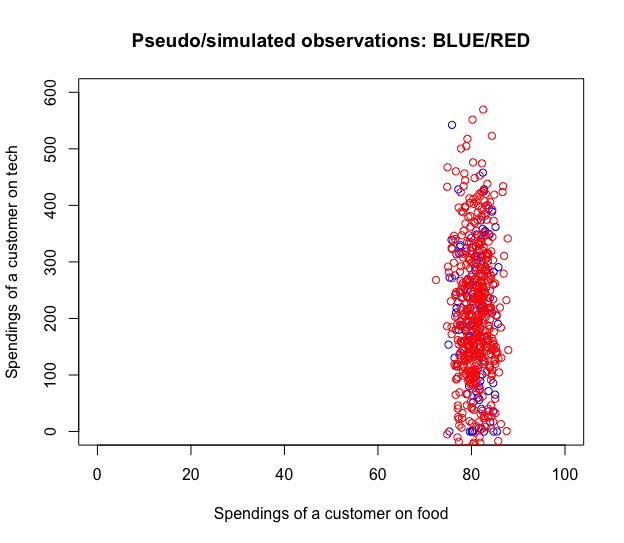
\includegraphics[width=0.6\textwidth]{uploads/upload_5818ee038f726ed6bde7bd783eb02212.png}
    \caption{Original and synthesized data for a particular functional of
interest.}
    \label{fig:copula_tech_vs_food}
\end{figure}

The main pitfall of copulas though is that this approach does not
provide a user-friendly tool to impose some additional constraints on
the generation process. For example, it seems imposible to generate the
data following the distribution of the original data with an additional
constraint of the data to sum up to a particular number. Yet this
constraint may become very critical in applications.

\subsection{Autoencoders}\label{autoencoders}

Autoencoders is a simple artificial neural network used to generate data
that look alike the original data. It is schematically illustrated in
the following Figure.

\begin{figure}
    \centering
    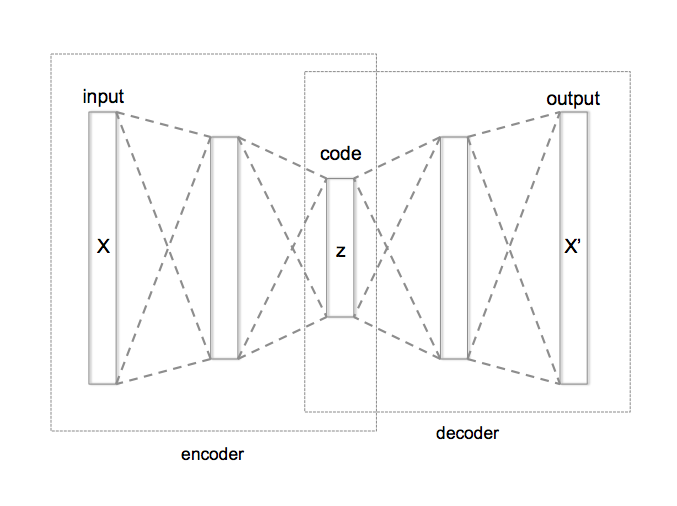
\includegraphics[width=0.8\textwidth]{uploads/upload_155f5da53a718fb42fa123c51e721762.png}
    \caption{Variational Autoencoder}
    \label{fig:autoencoder}
\end{figure}

The autoencoder above is called contractive as it has a ``bottleneck''
in the middle that stores the information about the original data
through some functionals. Once fully trained, only the value of the
functional is required to generate the output data. An autoencoder
always consists of two transition functions \(\psi, \phi\) and is very
suitable to answer the following questions:

\begin{itemize}
\tightlist
\item
  The original data are given and the objective is to generate data that
  look alike the original data.
\item
  The original data and a functional are given and the task is to
  synthetise data such that the functional evaluated on the generated
  data has a similar value as the functional evaluated on the original
  data.
\item
  Only functionals of the original data are given and the task is to
  generate data that yield similar values of the functionals
\end{itemize}

Formally, it solves the following optimisation problem
\[\phi :{\mathcal {X}}\rightarrow {\mathcal {F}} \\
\psi :{\mathcal {F}} \rightarrow {\mathcal {X}} \\
\phi, \psi = \arg\min_{\phi , \psi} \|X -  (\psi \circ \phi) X \|^2\]

Depending on the scenario of interest this optimisation scheme may
expand. For example, in order to generate data such that a given
functional evaluated on the data coincides with the functional on the
original data we solve the following optimisation problem.

\begin{figure}
    \centering
    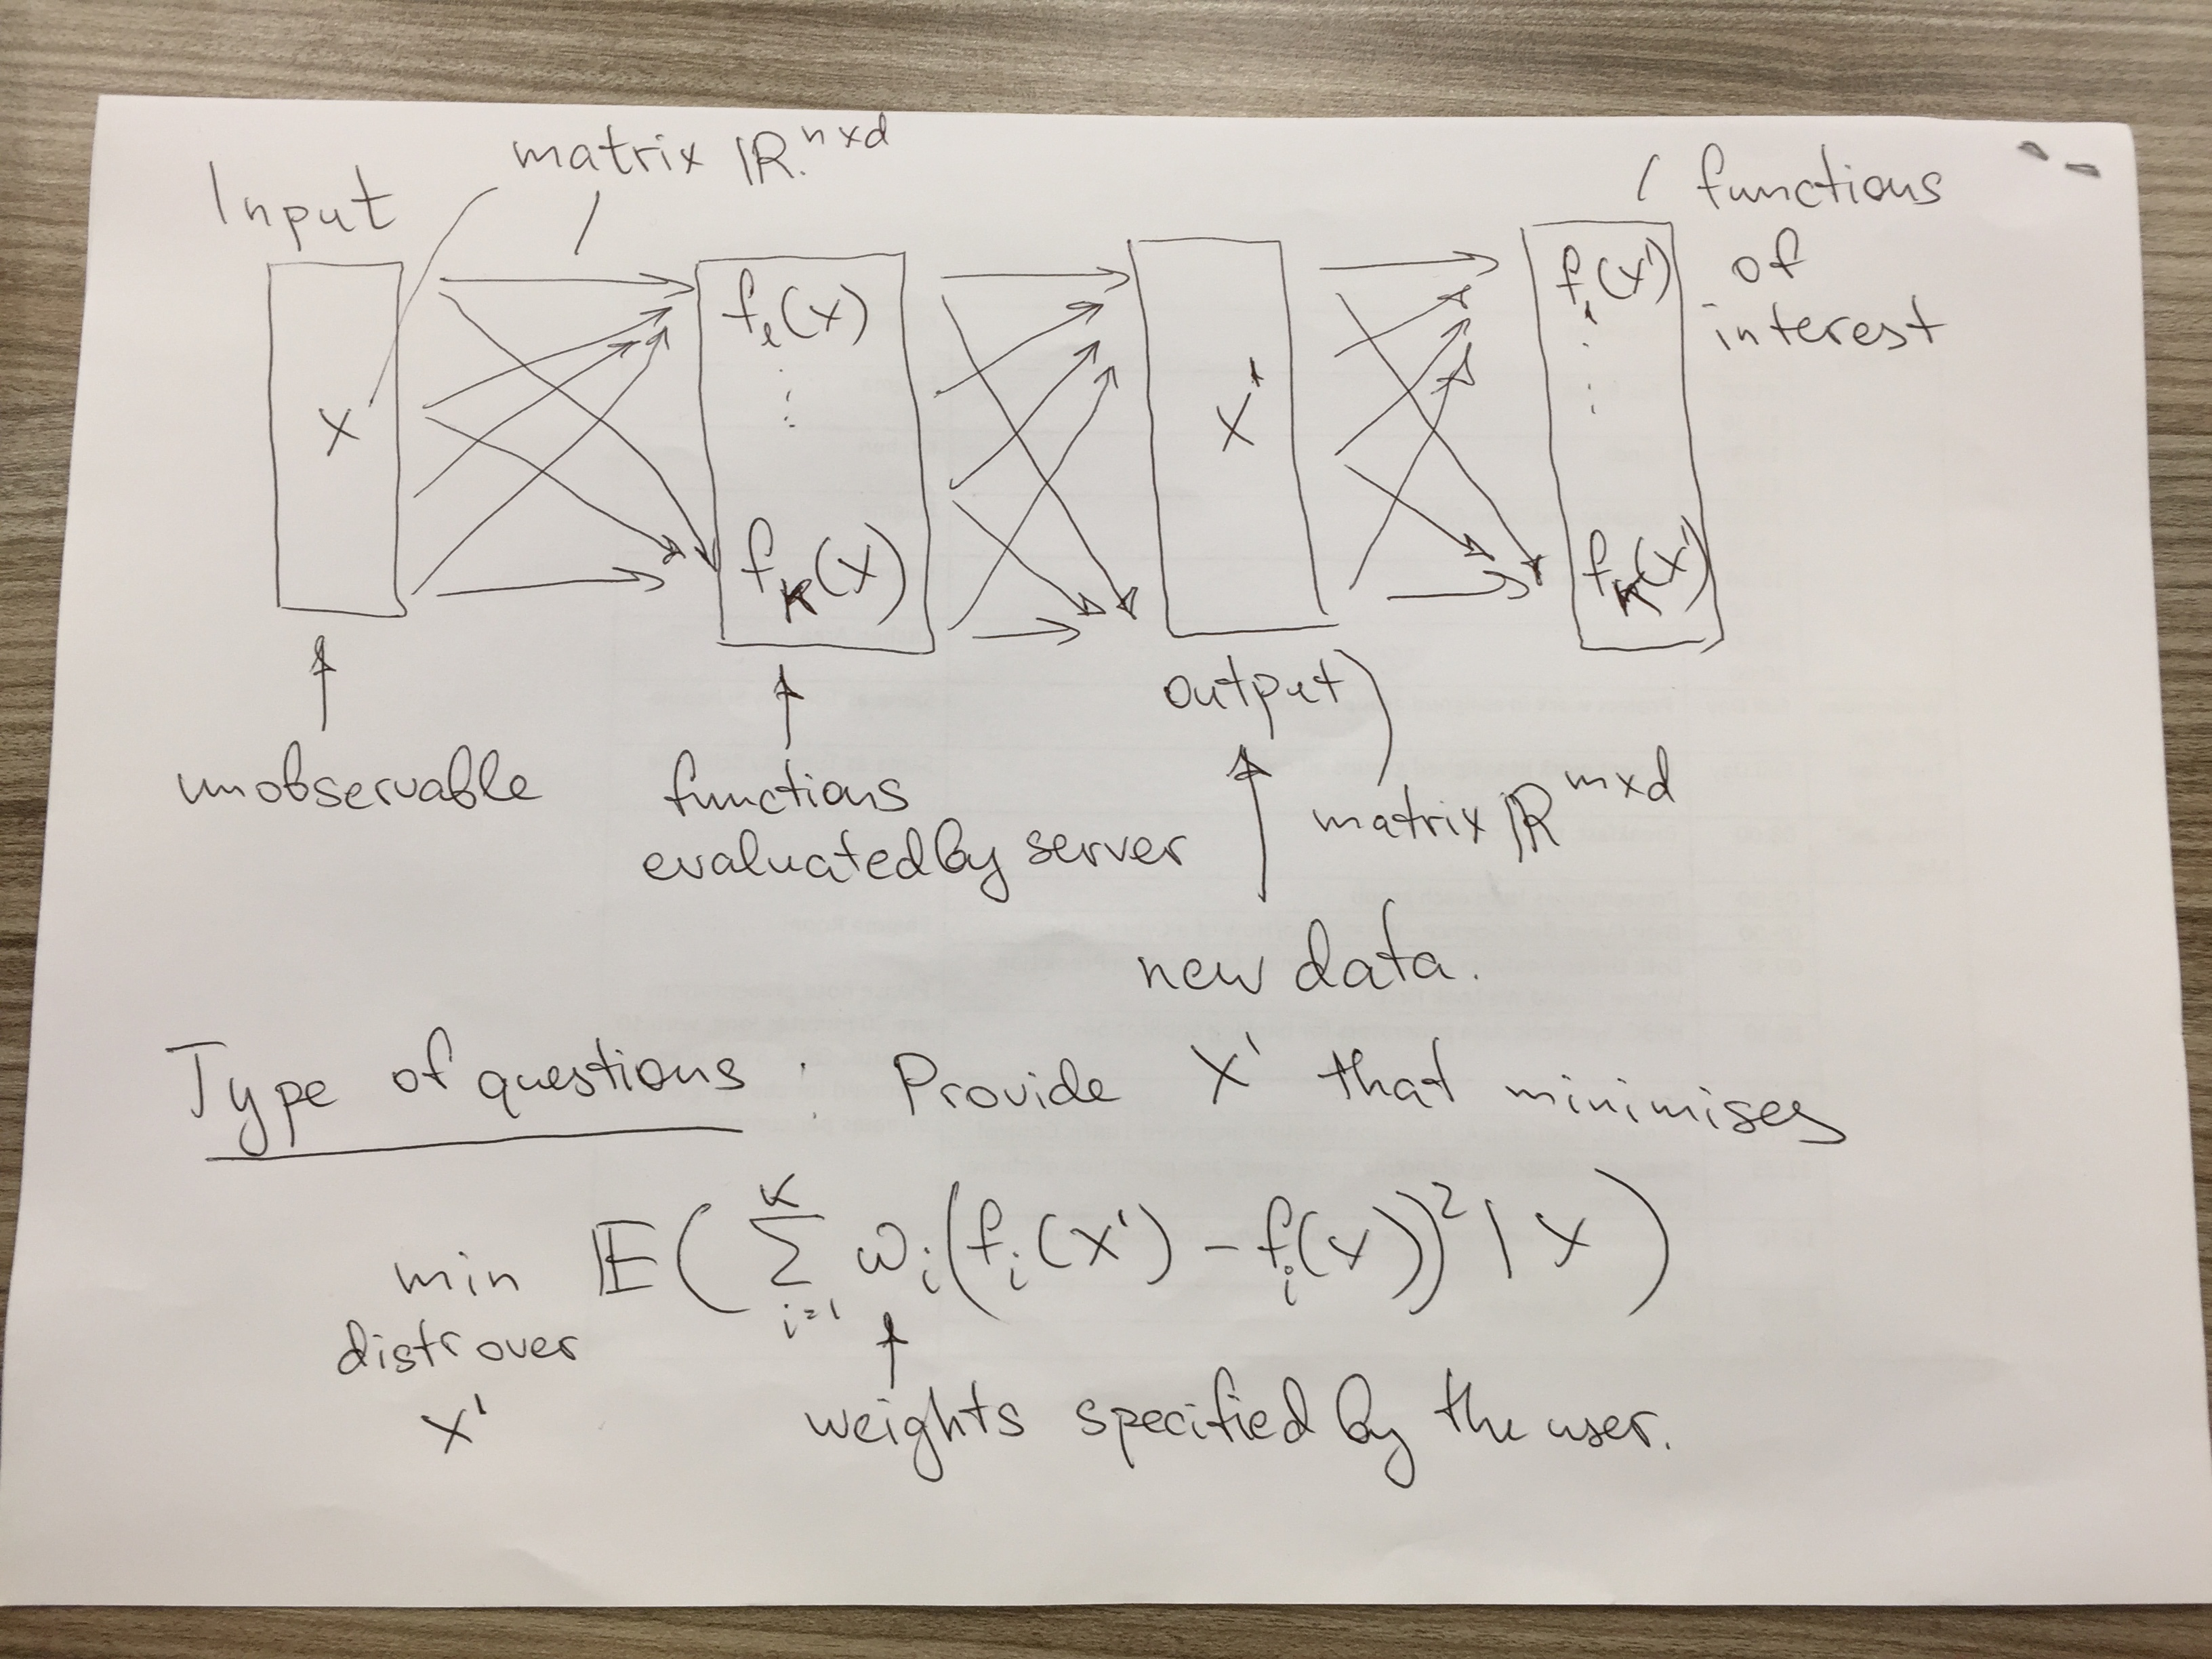
\includegraphics[width=0.8\textwidth]{uploads/upload_90956042bc74308a6b58ab8792c7593a.JPG}
    \caption{Targeted Autoencoder}
    \label{fig:autoencoder_sketch}
\end{figure}


\section{Conclusion}\label{conclusion}

Even though the formulation of the problem is quite general, it seems to
break down into a few fairly orthogonal scenarios. The data generation
process may or may not depend on the questions asked to the data set. In
a simple scenario, the data generation process is independent of
research questions and the task is to learn a generative model of the
data. For this scenario, we have mostly exploited Bayesian probabilistic
modeling. Not surprisingly, the model becomes high-dimensional and
fairly hard to train. Nevertheless, the data may be generally
applicable, and can respond to different applications by choice of rules
in the ABM environment. The resultant data is not likely to suffer
significant privacy concerns. The main drawback though is that there is
no guarantee that it is going to be useful to answer specific research
questions. For example, the current model generates time series by rules
imposed in the ABM rather than encoding the trends in the data.
Furthermore it is not really clear how to incorporate the randomness in
the number of customers into this model.

In another scenario, the aim is to synthetise data that answers a
specific range of research questions and satisfies some constraints. An
example is a data generator that synthesizes data with the same
cumulative spendings in a given time period. It does not necessarily
produce the same number of customers and even the distribution of the
data may be significantly different from the distribution of the
original data. In essence, it permits an answer only to those research
questions that are stated beforehand. On the other hand, it is fairly
flexible and seems to easily circumvent legal and privacy issues. For
example, the following data generated from the original data in Table in
Section 2.3.2 clearly allows to model the spendings in two sectors on a
particular date in a particular location.

\begin{longtable}[]{@{}ccccc@{}}
\toprule
ID & location & money spent on tech & money spent on food &
date\tabularnewline
\midrule
\endhead
2 & cb2 & 5000 & 500 & 1\tabularnewline
3 & cb2 & 40 & 2 & 13\tabularnewline
3 & cb2 & 13000 & 200 & 1\tabularnewline
4 & cb2 & 60 & 4 & 13\tabularnewline
3 & cb2 & 2000 & 300 & 1\tabularnewline
\ldots{} & \ldots{} & \ldots{} & \ldots{} & \ldots{}\tabularnewline
\bottomrule
\end{longtable}

Another important component of the data generation process is the
validation of the results. We face a standard problem of overfitting:
more complex models tend to mimic the data exactly and are hence
unsutiable for research in view of privacy issues whereas the output of
simple models is not very viable. Furthermore, some components of the
original data may be more sensitive than the others. It is an open
problem to incorporate these sensitive parameters as constraints into
the data generation process and then validate the security and
intergrity of the generated data.

\subsection{References}\label{references}
** NEEDS TO BE SUBSUMED INTO BIBLIOGRAPHY **
{[}1{]} E. Bonabeau, ``Agent-based modeling: methods and techniques for
simulating human systems.,'' Proc. Natl. Acad. Sci., vol.~99, no. suppl.
3, pp.~7280--7287, 2002. {[}2{]} N. Huynh, M. Namazi-Rad, P. Perez, M.
J. Berryman, Q. Chen, and J. Barthelemy, ``Generating a Synthetic
Population in Support of Agent- Based Modeling of Transportation in
Sydney Huynh et al., Generating a Synthetic Population in Support of
Agent-Based Modelling of Transportation in Sydney,'' pp.~1--6, 2013.
{[}3{]} G. Toscani and L. Pareschi, ``Wealth distribution and collective
knowledge: a Boltzmann approach.'' {[}4{]} L. F. Perrone, F. P. Wieland,
J. Liu, B. G. Lawson, D. M. Nicol, and R. M. Fujimoto, ``tutorial on
agent-based modeling and simulation part 2: how to model with agents.''
{[}5{]} ``Agent-based\_model.'' . {[}6{]} E. Bonabeau, ``Agent-based
modeling: Methods and techniques for simulating human systems.'' {[}7{]}
C. M. M. M. J. North, ``Tutorial on agent based modelling.'' {[}8{]}
``Mesa 0.8.0\,: Python Package Index.'' {[}Online{]}. Available:
https://pypi.python.org/pypi/Mesa/. {[}Accessed: 25-May-2017{]}. {[}9{]}
``Introductory Tutorial --- Mesa .1 documentation.'' {[}Online{]}.
Available:
http://mesa.readthedocs.io/en/latest/tutorials/intro\_tutorial.html\#setting-up-the-model.
{[}Accessed: 25-May-2017{]}. {[}10{]} A. Gosavi. Simulation-Based
Optimization: Parametric Optimization Techniques and Re-inforcement
Learning, Springer, New York, NY, Second edition, 2014 {[}11{]} Tutorial
on Reinforcement Learning {[}Online{]}
https://www.nervanasys.com/demystifying-deep-reinforcement-learning/

\subsection{8. Bibliography}\label{bibliography}

\begin{itemize}
\tightlist
\item
  \href{http://lisp.vse.cz/pkdd99/berka.htm}{PKDD'99 dataset}
\item
  \href{https://www.europeandataportal.eu/data/en/dataset/corporate-credit-card-transaction-2014-15}{UK
  Government Company Credit Card records 2014-2015}
\item
  \href{https://www.europeandataportal.eu/data/en/dataset/corporate-credit-card-transactions-2015-16}{UK
  Government Company Credit Card records 2015-2016}
\item
  \href{http://dai.lids.mit.edu/pdf/SDV2.pdf}{Patki, N.; Wedge, R.;
  Veeramachaneni, K. (2016) The Synthetic Data Vault. IEEE International
  Conference on Data Science and Advanced Analytics. Montreal, CA.}
\item
  \href{https://www.cis.upenn.edu/~aaroth/Papers/privacybook.pdf}{Dwork,
  C.; Roth, A. Foundations and Trend in Theoretical Computer Science.
  Vol. 9, Nos. 3--4 (2014) 211--407. 2014}
\end{itemize}

\bibliographystyle{abbrvnat}
\bibliography{biblio}

\subsection{Appendix}\label{appendix}

\subsubsection{Tables for variable
encoding}\label{tables-for-variable-encoding}

\begin{longtable}[]{@{}lc@{}}
\toprule
Category description & Code\tabularnewline
\midrule
\endhead
Advertising & 0\tabularnewline
Books-CDs-Audio-Video & 1\tabularnewline
Building Repairs \& Maintenance & 2\tabularnewline
Cleaning and domestic material & 3\tabularnewline
Clothing - Protective Clothing & 4\tabularnewline
Clothing - Uniforms & 5\tabularnewline
Conference Expenses & 6\tabularnewline
Consumable Catering Supplies & 7\tabularnewline
Counsels Fees & 8\tabularnewline
E19 - Learning Resources & 9\tabularnewline
E25 - Catering Supplies & 10\tabularnewline
Education CFR Administrative S & 11\tabularnewline
Education CFR Other Occupation & 12\tabularnewline
Electricity & 13\tabularnewline
Employer's National Insurance & 14\tabularnewline
Equipment and Materials Purcha & 15\tabularnewline
Equipment and Materials Repair & 16\tabularnewline
Fees and Charges & 17\tabularnewline
Food Costs & 18\tabularnewline
Furniture-Purchase-Repair & 19\tabularnewline
General Office Expenses & 20\tabularnewline
Grant Payments & 21\tabularnewline
Grounds maintenance & 22\tabularnewline
Hardware Purchases & 23\tabularnewline
IT Services & 24\tabularnewline
Legal and Court Fees & 25\tabularnewline
Miscellaneous Expenses & 26\tabularnewline
Operating Leases - Transport & 27\tabularnewline
Other Agencies - Third Party P & 28\tabularnewline
Other Energy & 29\tabularnewline
Other Establishments - Third P & 30\tabularnewline
Other Indirect Employee Expens & 31\tabularnewline
Other Services & 32\tabularnewline
Other Transfer Payments to Soc & 33\tabularnewline
Other Vehicle Costs & 34\tabularnewline
Pool Transport Charges & 35\tabularnewline
Postage & 36\tabularnewline
Printing-Contract & 37\tabularnewline
Private Contractors - Third Pa & 38\tabularnewline
Professional Services & 39\tabularnewline
Publications & 40\tabularnewline
Software Licences \& Support & 41\tabularnewline
Stationery & 42\tabularnewline
Subscriptions & 43\tabularnewline
Subsistence & 44\tabularnewline
Telephone Rentals & 45\tabularnewline
Telephones Calls & 46\tabularnewline
Training & 47\tabularnewline
Transport Hire Charges & 48\tabularnewline
Travelling Expenses & 49\tabularnewline
Vehicle Running Costs & 50\tabularnewline
Venue Hire & 51\tabularnewline
Water Services & 52\tabularnewline
\bottomrule
\end{longtable}

\begin{longtable}[]{@{}cc@{}}
\toprule
Operation & Code\tabularnewline
\midrule
\endhead
Withdrawal & 0\tabularnewline
Deposit & 1\tabularnewline
\bottomrule
\end{longtable}

\begin{longtable}[]{@{}cc@{}}
\toprule
Type of transaction & Code\tabularnewline
\midrule
\endhead
Bank remittance & 0\tabularnewline
Bank collection & 1\tabularnewline
Credit in cash & 2\tabularnewline
Cash withdraw & 3\tabularnewline
Card withdraw & 4\tabularnewline
\bottomrule
\end{longtable}

\begin{longtable}[]{@{}cc@{}}
\toprule
Frequency & Code\tabularnewline
\midrule
\endhead
After each Transaction & 1\tabularnewline
Weekly & 2\tabularnewline
Monthly & 0\tabularnewline
\bottomrule
\end{longtable}

\begin{longtable}[]{@{}cc@{}}
\toprule
K-symbol & Code\tabularnewline
\midrule
\endhead
Insurance payment & 0\tabularnewline
Statement payment & 1\tabularnewline
Interest credited & 2\tabularnewline
Overdraft penalty & 3\tabularnewline
Household payment & 4\tabularnewline
Pension & 5\tabularnewline
Loan payment & 6\tabularnewline
\bottomrule
\end{longtable}

\subsection{Appendix II : Sample Synthetic Data Generated using
ABMs}\label{appendix-ii-sample-synthetic-data-generated-using-abms}

\begin{figure}
\centering
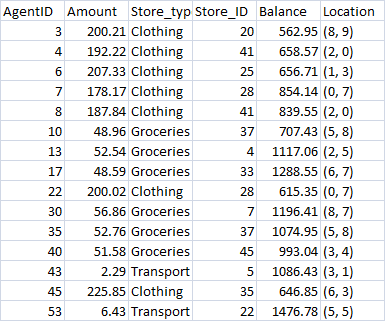
\includegraphics{uploads/upload_22258fd69d3fe4f27d9cd3a423fc7650.png}
\caption{}
\end{figure}


\end{document}
